\infoleveqnull{\section{Hall C Spectrometers}}
%\section{Introduction}

	The two magnetic spectrometers in Hall~C are designed to perform
high resolution and high accuracy nuclear physics experiments.  These
spectrometers transport and detect charged particles that are scattered or produced 
in beam-target interactions.
\infolevone{
In this chapter
we discuss the features and safe operation of these spectrometers,
the High Momentum Spectrometer, or HMS,
and Super High Momentum Spectrometer, or SHMS.  These spectrometers
share many common features.  After this
introduction and overviews of the individual spectrometers, the
spectrometers are discussed together as a series of subsystems.
This chapter covers the ``mechanical'' subsystems of the spectrometers.
The detector packages and
shield houses are discussed in Chapter~\ref{chap:detectors}.

Both the HMS and the SHMS are designed around a series of superconducting magnets,
including quadrupoles and dipoles, followed by a set of particle detectors.  The first
magnet on the SHMS is a horizontal-bending (HB) dipole that bends particles
away from the beam-line. The HMS does not have a horizontal bender.
The primary purpose of the quadrupole magnets is to increase the flux of
charged particles entering the main dipole magnets and to focus the orbits of the
charged particles into the detector huts.
The dipole magnets deflect charged particles vertically
as they enter the detector hut. Some of the detectors measure the amount of deflection
so that we may
determine the momentum of each particle. Other detectors provide accurate timing 
to trigger the readout of all detector data, or they measure a particle's speed
or total energy so that we can determine its mass.

Each spectrometer is built on a rotatable support structure or carriage. 
These ride on steel 
wheels and rails and rotate around the pivot. Experiments using the HMS or
SHMS place their experimental targets along the beamline above the pivot.
The support structures carry the weight of the magnets and detectors, and keep
them aligned to one-another and pointed at the target. On the SHMS, the shield 
house and all of the
other spectrometer equipment are also carried by the support structure. The
HMS has a separate carriage that supports these items.

During beam operations a large number of particles is
produced in the target. A few of these enter one of the spectrometers. Most of 
them go forward at small angles and are stopped in the beam dump. The
remainder, scattered over a wide range of angles,  interact with the beam pipe, 
the air, nearby structures, etc., and
constitute background radiation that would overwhelm the detectors.
The shield houses have thick walls that are designed to reduce the amount of
radiation that gets inside. Both spectrometers use
concrete and lead lining on the walls as shielding. On
the SHMS, two custom types of concrete improve the neutron stopping power 
of the walls by
adding boron (in the form of boron-carbide) or extra hydrogen (recycled
plastic chips). Each shield house has a room that surrounds the detectors.
The SHMS has a second room, shielded from the first, that protects the
electronic systems.

%Each spectrometer includes a shield house which contain the particle
%detector packages.  In the case of the SHMS, this shield house (and a separate
%shield house for electronics) are part of the carriage structure.  In
%the case of the HMS, the detector shield house is a separate
%structure, coupled to the carriage by a ``push bar'' on the ``pasta fork''.
%The ``pasta fork" is the name given to the steel piece that protrudes
%from the back of the carriage. The detector frame is supported on the
%``pasta fork." This insures that the detectors do not move relative
%to the magnetic elements.

\section{The High Momentum Spectrometer (HMS) }

10.5 to 90 degrees.  Up to 7.4 geV/c.  

The HMS is composed of three superconducting quadrupole magnets,
Q1, Q2, and Q3, and one superconducting dipole magnet. The quadrupoles
were manufactured for JLab by {\em OXFORD} while the dipole was built for 
JLab by {\em ELIN}.
The quadrupole magnets are referred to as Q1, Q2, and Q3, where a particle first traverses 
Q1, then Q2 and Q3, and finally traverses the dipole magnet.

The magnet system is followed by a large concrete detector hut, in which all
detector elements reside. The main fraction of the detector elements have been
built by universities involved in the Hall~C physics program.

The HMS magnet system is the cornerstone of the Hall~C activities.
Many of the experiments approved in Hall~C center on physics at high
momentum transfers and other short-range phenomena, and rely on a spectrometer
able to momentum analyze charged particles up to very high momenta.
The design value for the maximum momentum accessible to the HMS magnet
system is 6 GeV/c, though in its initial phase the maximum momentum
has been limited to 4 GeV/c.


\section{The Super High Momentum Spectrometer (SHMS)}
%5.5 to 40 degrees.  Up to 11 GeV/c.  
%
%The purpose of the SHMS horizontal bender is to bend scattered
%particles away from the beamline so that smaller scattering angles can be
%measured.
The Super High Momentum Spectrometer (SHMS) operates on the beam-left
side of the beamline, and can be rotated around the pivot for scattering angles from 5.5
to 40~degrees. It was built between 2009 and 2016 as the major
Hall-C component of the 12-GeV Upgrade Project.  The five superconducting
magnets on the SHMS can be set for a central-ray momentum of up to 11~GeV/c.
The minimum design momentum is 2 GeV/c. A CAD model of the SHMS is shown
in Fig.~\ref{fig:SHMS_CAD_Model} and Table y??y lists the performance specifications. 

\begin{figure}
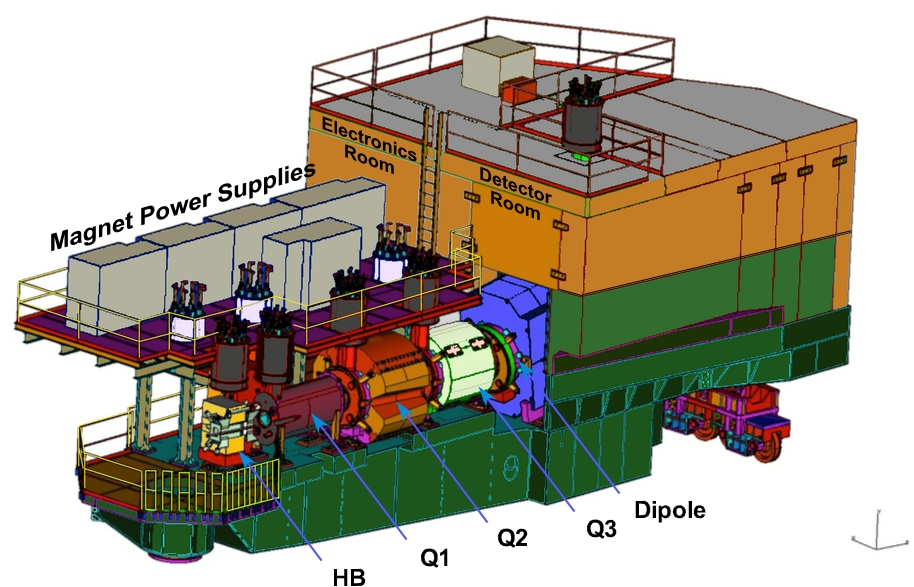
\includegraphics[width=6in]{SHMS_Rendered_Recolored_Annotated}
\caption{CAD Rendering of the Super-High-Momentum Spectrometer. \label{fig:SHMS_CAD_Model}}
\end{figure}

The primary magnetic elements on the SHMS, the Q1, Q2, Q3, and Dipole magnets, provide
point-to-point focusing and momentum dispersion just like the four magnets with
the same names on the HMS. The SHMS Q1 was 
manufactured by Scientific Magnetics, Inc. in Abingdon, England. The Q2, Q3, and
the Dipole were constructed by Sigmaphi in Vannes, France.

In order to reach the smallest scattering angles the SHMS has a horizontal-bend
(HB) magnet as its first magnetic element. It was built by FRIB, the Department of Energy
facility at Michigan State  University. This small, high-field magnet bends
central-momentum particles to the left by 3~degrees so that the remainder of the
spectrometer parts will be further away from the primary electron beam. The HB
magnet is an asymmetric "C"-dipole which has a flux-return iron yoke only on
the side away from the primary beam. When the SHMS is set for small scattering 
angles, the electron beam passes very close to the spectrometer and to the
HB magnet's superconducting
coils. In this configuration the coils see a high radiation dose which may cause
them to have a limited 
lifetime. Experiments must be planned in such a way that this exposure is minimized.

A further consequence of making the SHMS operate at small scattering angles is
that the iron yokes of the HB and Q2 magnets had to be designed with notches 
that just clear the beamline vacuum pipe. The fringe fields from these magnets can
deflect the primary electron beam away from the middle of the beam dump. 
The effects of this field
must be mitigated by a combination of good experiment planning, magnetic shielding, 
and automatic safety systems.

The SHMS shield house has two rooms. The dipole magnet penetrates the front
wall of the room containing the detectors. Inside this are the two sets of 6-plane
drift chambers, the Heavy-Gas Cerenkov (HGC), the two pairs of trigger hodoscopes 
(S1X/S1Y and S2X/Q2Y), and
the Preshower and Shower Counters (calorimeters). The SHMS focal plane forms an 
angle of about 5~degrees with respect to the central trajectory, 
and intersects that trajectory at
a point midway between the two drift chamber boxes. Additional  particle-identification
detectors (Noble-Gas Cerenkov (NGC), and/or Aerogel Cerenkov) may also be 
installed if needed by the current experiment. When the NGC is not in use it may
be replaced by a tank that extends the vacuum system up  to a window just in
front of the first drift chamber. In this configuration, a mechanical safety shutter
must be closed over this large vacuum window before personnel may enter the
room.

The second room in the SHMS shield house houses the
electronics controlling the magnet power supplies, the data-acquisition 
electronics (DAQ) and power supplies for the detectors, and theVESDA
smoke and flammable gas sensor systems. When personnel enter the shield
house they first pass into this "Electronics Room". 
}

\begin{safetyen}{0}{0}
\infolevone{\section{Safety Information}}
\label{sec:hrs-safety}

\subsection{Hazards}

The spectrometers have associated vacuum, electrical, cryogenic and
magnet systems all of which can be extremely dangerous due to the size
and stored energy in the systems.  
Parts of the spectrometers are at elevated levels which would present fall
hazards if the installed safety equipment were not present.
Hazards of rotating the
spectrometers as well as the particle detectors that get placed inside
the detector hut of the spectrometer are covered in detail in
following sections.

Signage and alerts are placed to remind workers of some of the potential hazards
in Hall C, but each individual is ultimately responsible for his or her own 
safety. Always read and respect warning signs, and never attempt to 
circumvent barriers or other equipment
that has been installed for your protection. If you discover what appears to be a
new or unidentified hazard, protect your coworkers by warning them
and alert the Hall-C management and Safety Warden.

\subsection{Mitigations}

Both of the spectrometers have elevated work platforms that are secured by
gates and handrails. Never attempt to bypass these protections. During experiment
running periods, in order to allow spectrometer rotation, it may be necessary to
remove the handrails around the target platform. In this condition access to the 
target platform is restricted to trained individuals who have been specifically
authorized to work near there. Fall-protection equipment is required.

The vacuum systems associated with the spectrometers are essentially 
pressure vessels and care should be exercised so as not to damage or puncture the 
vacuum windows.   The large vacuum windows inside the two shield houses are protected
by shutters which must be lowered into place before the access door to the
detector rooms will open. (When the Noble-Gas Cerenkov (NGC) is installed in the SHMS, 
the NGC itself protects the vacuum window and the shutter is not present.)
During hall maintenance, covers are placed over the spectrometer
vacuum windows near the pivot
to help prevent anything from accidentally hitting a window.

The magnets themselves are installed inside cryostats.  These vessels 
are exposed to high pressures and are therefore equipped with safety 
relief valves and burst discs.   

The cryogenic system operates at an elevated pressure and at a temperature 
about 4~Kelvin (helium system) or about 90~Kelvin (nitrogen system).  One must
guard against cold burns and take the normal precautions with pressure
vessels when operating this system.  Manipulation of any cryogenic system
component such as a U-Tube or manual valve may only be performed by
a trained cryogenic-system expert.

When they are powered, the magnets have a great deal of stored energy as they are large 
inductors. Always make sure people are clear of the magnets and their dump resistors.

\subsection{Responsible Personnel}

In the event that problems arise during 
operation of the magnets, qualified personnel should be notified
(see Table \ref{tab:spec:personnel_magnet}).  
This includes any prolonged or serious problem with the source of magnet 
cryogens (the ESR).  On weekends and after hours there will be a 
designated individual on call for magnet services.  Any member of the 
Hall A technical staff is qualified to deal with unusual magnet 
situations but in the event of serious problems the technician on
call should be contacted.

\begin{namestab}{tab:spec:personnel_magnet}{Spectrometers: authorized personnel}{%
      List of spectrometer responsible personnel where ``W.B.'' stands for the white board 
      in the counting house.}
   \TechonCall{\em Contact}
   \PaulBrindza{}
   \SteveLassiter{}
   \EricSun{}
   \MikeFowler{}
   \JoeBeaufait{}
   \JackSegal{}
   \MahlonLong{}
\end{namestab}


\end{safetyen}

\infolevone{
\section{Features Common to Both Spectrometers}

\subsection{Vacuum Windows}

\paragraph{Overview}

Because multiple scattering degrades the performance of a spectrometer, it is
important that the spectrometer volume be evacuated and that the vacuum
entrance and exit windows
be as low mass as possible. However,
catastrophic window failure would generate a significant shock wave as air
rushed to fill the vacuum volume. It would also cause a loud noise which
could cause hearing damage to anyone in the immediate vicinity.
The material chosen for the vacuum windows, then, must be both light enough
to have a minimum effect on the beam and
strong enough to operate reliably and safely.

The HMS spectrometer vacuum channel has a volume
of approximately $6$ m$^3$, representing a stored energy of $6 \times 10^5$
Joules. A drawing of the  flange to which the exit vacuum
window is attached is shown in Figure~\ref{fig:hms_flange}.  It is a
circle with a center-to-center bolt hole diameter of $40$ inches
and a $38$ inch diameter opening. This is the largest vacuum window
required for Hall~C.
Under vacuum, this window must support 16,785
lbs (74,425 N). It is located in the HMS detector hut. 

In the past, prior to the 12-GeV Upgrade, multiple scattering was a
more significant issue than it is with today's higher-energy particles.  
The large  vacuum window in the HMS
shield house was often made of a Mylar/Kevlar composite material. 
The density of the Kevlar used was $\approx 0.75$ gm/cm$^3$ with a radiation
length of $55.2$ cm \cite{rdup1}. The radiation length
of Mylar is $28.7$ cm. The Kevlar has a tensile strength of 900 lbs/inch. This composite
material minimized the effective thickness of the window while providing the needed
strength. However, the composite ages and loses integrity over time, so the window
had to be replaced approximately every six months. There is no longer any known
supplier of this material.

Thin metal windows have an indefinite lifetime and cause
multiple scattering which is small compared to the intrinsic resolution of
the Hall-C spectrometers. Both the HMS and the SHMS are now equipped
with metal windows, as detailed in Table ~\ref{tab:hall_c_windows_specs}.

\begin{table}
\begin{center}
\caption{Vacuum Windows in Hall C\label{tab:hall_c_windows_specs}}
\vspace{\baselineskip}
\begin{tabular}{|l|l|l|l|} 
\hline
Window Location				& Dimensions 	 	& Material & Thickness (mm) \\ \hline
Scattering Chamber Exit			& Very Wide		& Al		& 0.406\\
HMS Entrance	on Snout			& 254 mm (dia)		& Unob	& ??\\
HMS Exit						& 1016 mm (dia)	& Unob	& ??\\
SHMS Entrance on HB Magnet		& $\approx 180$(w) x $\approx 220$(h)		& Al	& 0.508\\
SHMS Exit					& 000 (dia)		& Al		& 0.508\\
SHMS Exit from Vacuum Extension	& 000 (dia)		& Al	& 0.508\\
\hline
\end{tabular}
\end{center}
\end{table}

As shown in the table, the entrance window to the HMS is on the end of the 
snout which extends from the HMS Q1 magnet towards the target. The SHMS
entrance window is on the front of the HB magnet. Fig.~\ref{fig:hms_flange} shows
the 8" long vacuum spool piece which forms the end of the HMS vacuum
volume and provides the mounting flange for the large vacuum window. 


%The HMS entrance window is located near the pivot and has a center-to-center
%bolt hole diameter of $10.5$ inches.

%Figure~\ref{fig:hms_flange}
\begin{figure}
\includegraphics[width=6in,trim=0 0 0 220bp,clip]{figHMSflange}
\caption{The HMS exit flange and the 8" long Vacuum Spool Piece. \label{fig:hms_flange}}
\end{figure}

\begin{obsolete}
The SOS spectrometer vacuum can has a volume of approximately $2$ m$^3$,
representing a stored energy of $2 \times 10^5$ Joules. The entrance
window (near the pivot) is round and has a diameter of $9$ inches.
The SOS exit window is the second largest window in Hall~C. This
window is located in the SOS detector hut. It is rectangular.
The opening has a length of $40.5$ inches and a width of $6.5$ inches.
The SOS exit
window must support a load of $3,896$ lbs ($17,275$ N) under vacuum.
\end{obsolete}

% Which responsible persons?
{\bf One of the responsible personnel must be present for
any work directly affecting a Hall~C vacuum window}.

\paragraph{Design and Placement of HMS Large Window}

\begin{obsolete}
After extensive testing of the above design
and of other similar designs and fabrics (Spectra, Kevlar/Nylon fabric),
we chose to have a new
material custom laminated for our purposes. The new window material is
composed of 0.015 inch ballistic Kevlar 29 style 713 (31x 31 count,
plain weave)
with 0.004 inch Mylar on
one side
and 0.001 inch thick Mylar on the other. Bolt holes are cut into the material
(using a custom made cutting tool) and it is then directly
mounted on a ring flange using standard O-ring vacuum
seal technique.  This material and
method have
been used successfully on both Hall~C spectrometers, holding a vacuum of
$\approx 10^{-4}$ Torr. It is necessary to have a large number of bolt holes in the flange ring
for clamping strength.
\end{obsolete}

Figures~\ref{fig:hms_window} shows the
window and ring flanges as mounted on the spectrometer. The thick
line represents the composite window. There are O-ring grooves on both the
ring flange for the window mount and on the spectrometer exit flange.
The ring flanges are rounded so as not to cut into the window fabric as
it bows under pressure.
For more detail on the window mounting, see
the section entitled ``Vacuum Window Installation Procedure", below.

\begin{figure}
\includegraphics[width=6in,trim=0 0 0 520bp,clip]{figHMSwindow}
\caption{The HMS vacuum window and ring flanges. \label{fig:hms_window}}
\end{figure}

Figure~\ref{fig:hms_window2} shows the window as placed in the HMS spectrometer
detector hut.
\begin{figure}
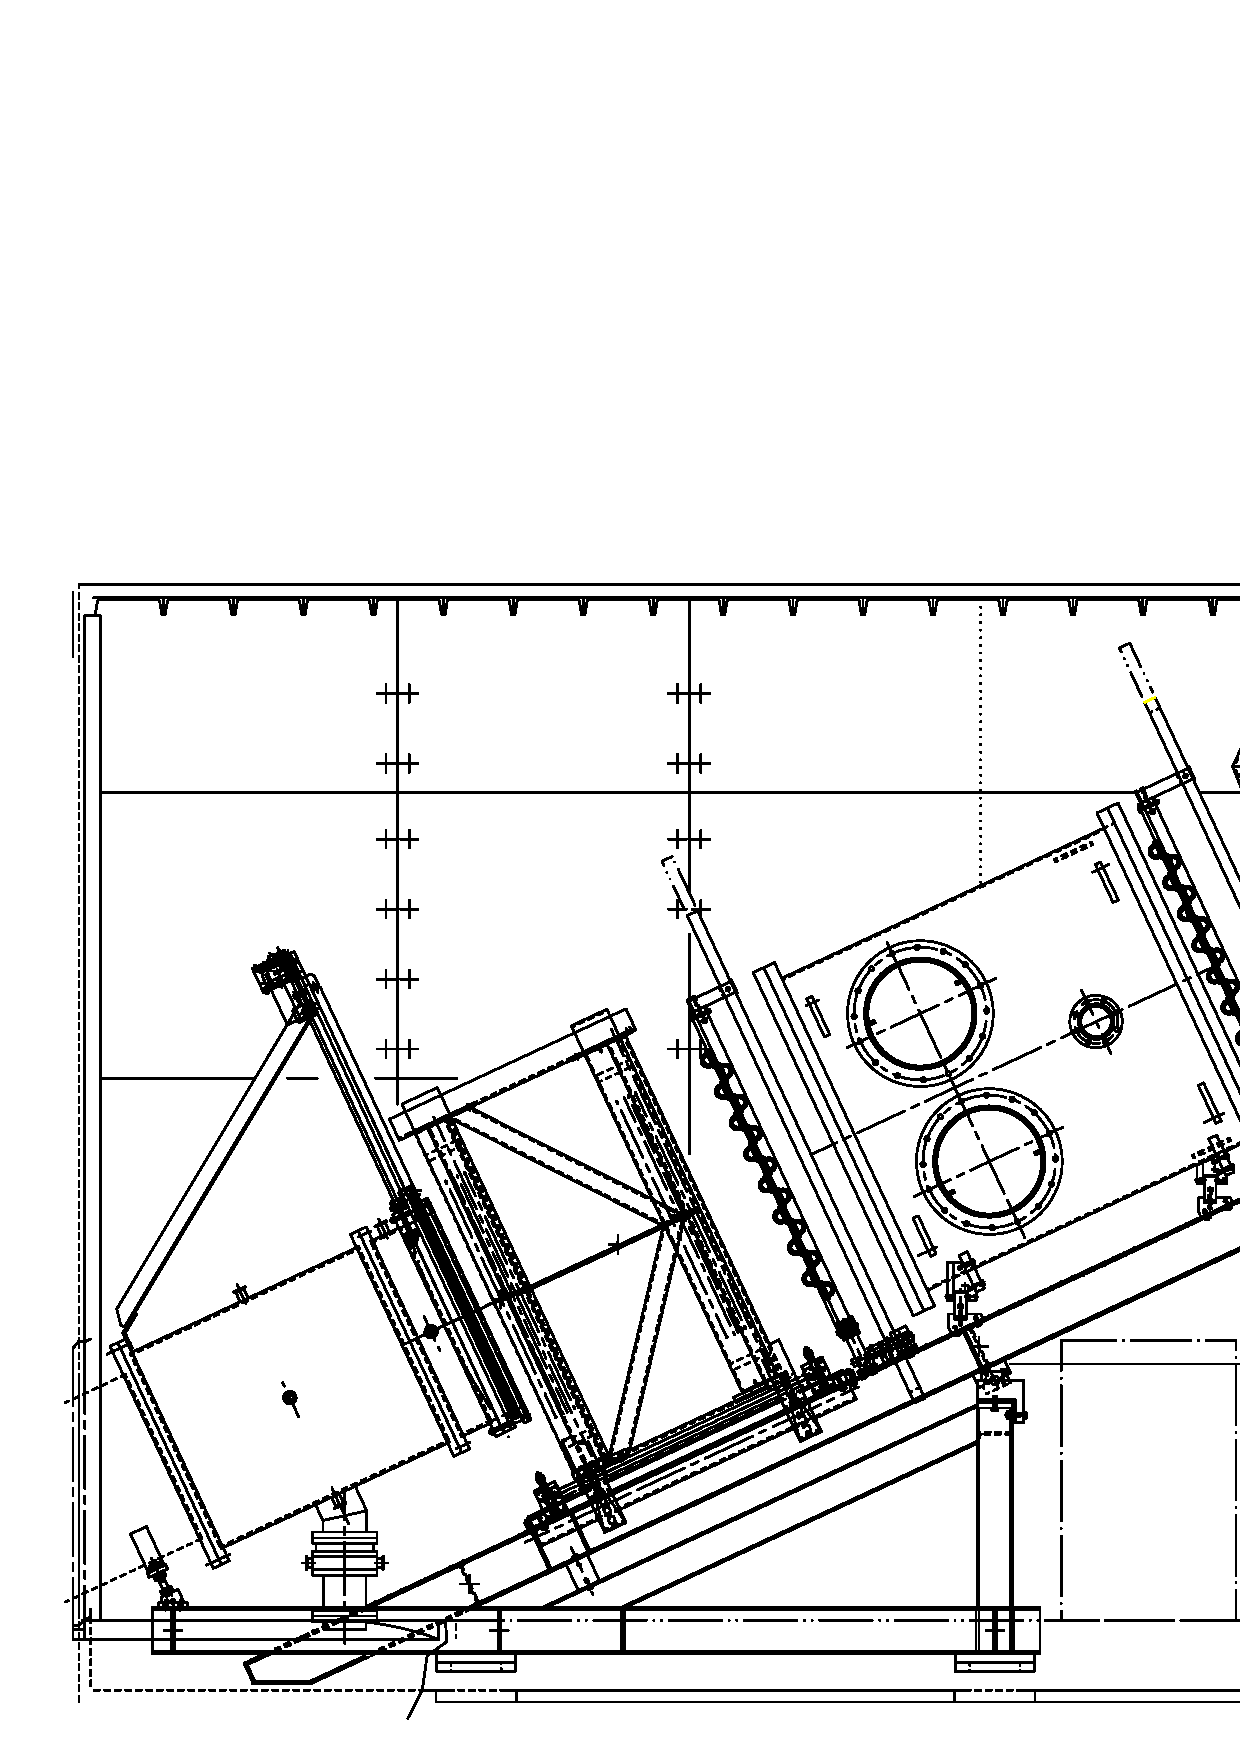
\includegraphics[width=6in,trim=0 0 0 230bp,clip]{figHMShut}
\caption{The HMS vacuum window in the HMS spectrometer hut. 
\label{fig:hms_window2}}
\end{figure}

The window (in its ring flanges) is mounted at the end of the $8$ inch
vacuum exit extension piece. The next element is an aluminum shutter which
must be lowered to cover the Mylar/Kevlar window whenever it is under
vacuum and personnel are working in the detector hut. The shutter
control panel is just outside the shielding house door, and an
indicator light signals whether the shutter is in or out.  

\paragraph{Other Windows}

The HMS spectrometer vacuum entrance is a $10.5$ inch (bolt circle) round
window. Presently, the entrance window
is made of the same laminate as the exit window. The
procedure for installation (see below) is also the same.
It is
also allowable to employ thinner Kevlar/Mylar
material for the HMS entrance window and for
the SOS spectrometer windows; a similar laminate as used in the
larger windows has been tested and utilized.  The thinner material is
composed of 0.0045'' Kevlar sandwiched between 2 sheets of 0.002'' Mylar.

\begin{obsolete}
The SOS spectrometer windows are currently made of the same composite fabric
as the HMS windows. The SOS exit window is rectangular, with a $6.5$ inch
by $39.5$ inch opening.
The window is cut out and installed with an O-ring as with the HMS
windows (see Figure~\ref{fig:hms_window}).
Because the maximum
loads under vacuum on the SOS windows (and HMS entrance window)
are much smaller than that on the HMS exit window,
there is
no aluminum shutter in the SOS spectrometer.

\begin{figure}
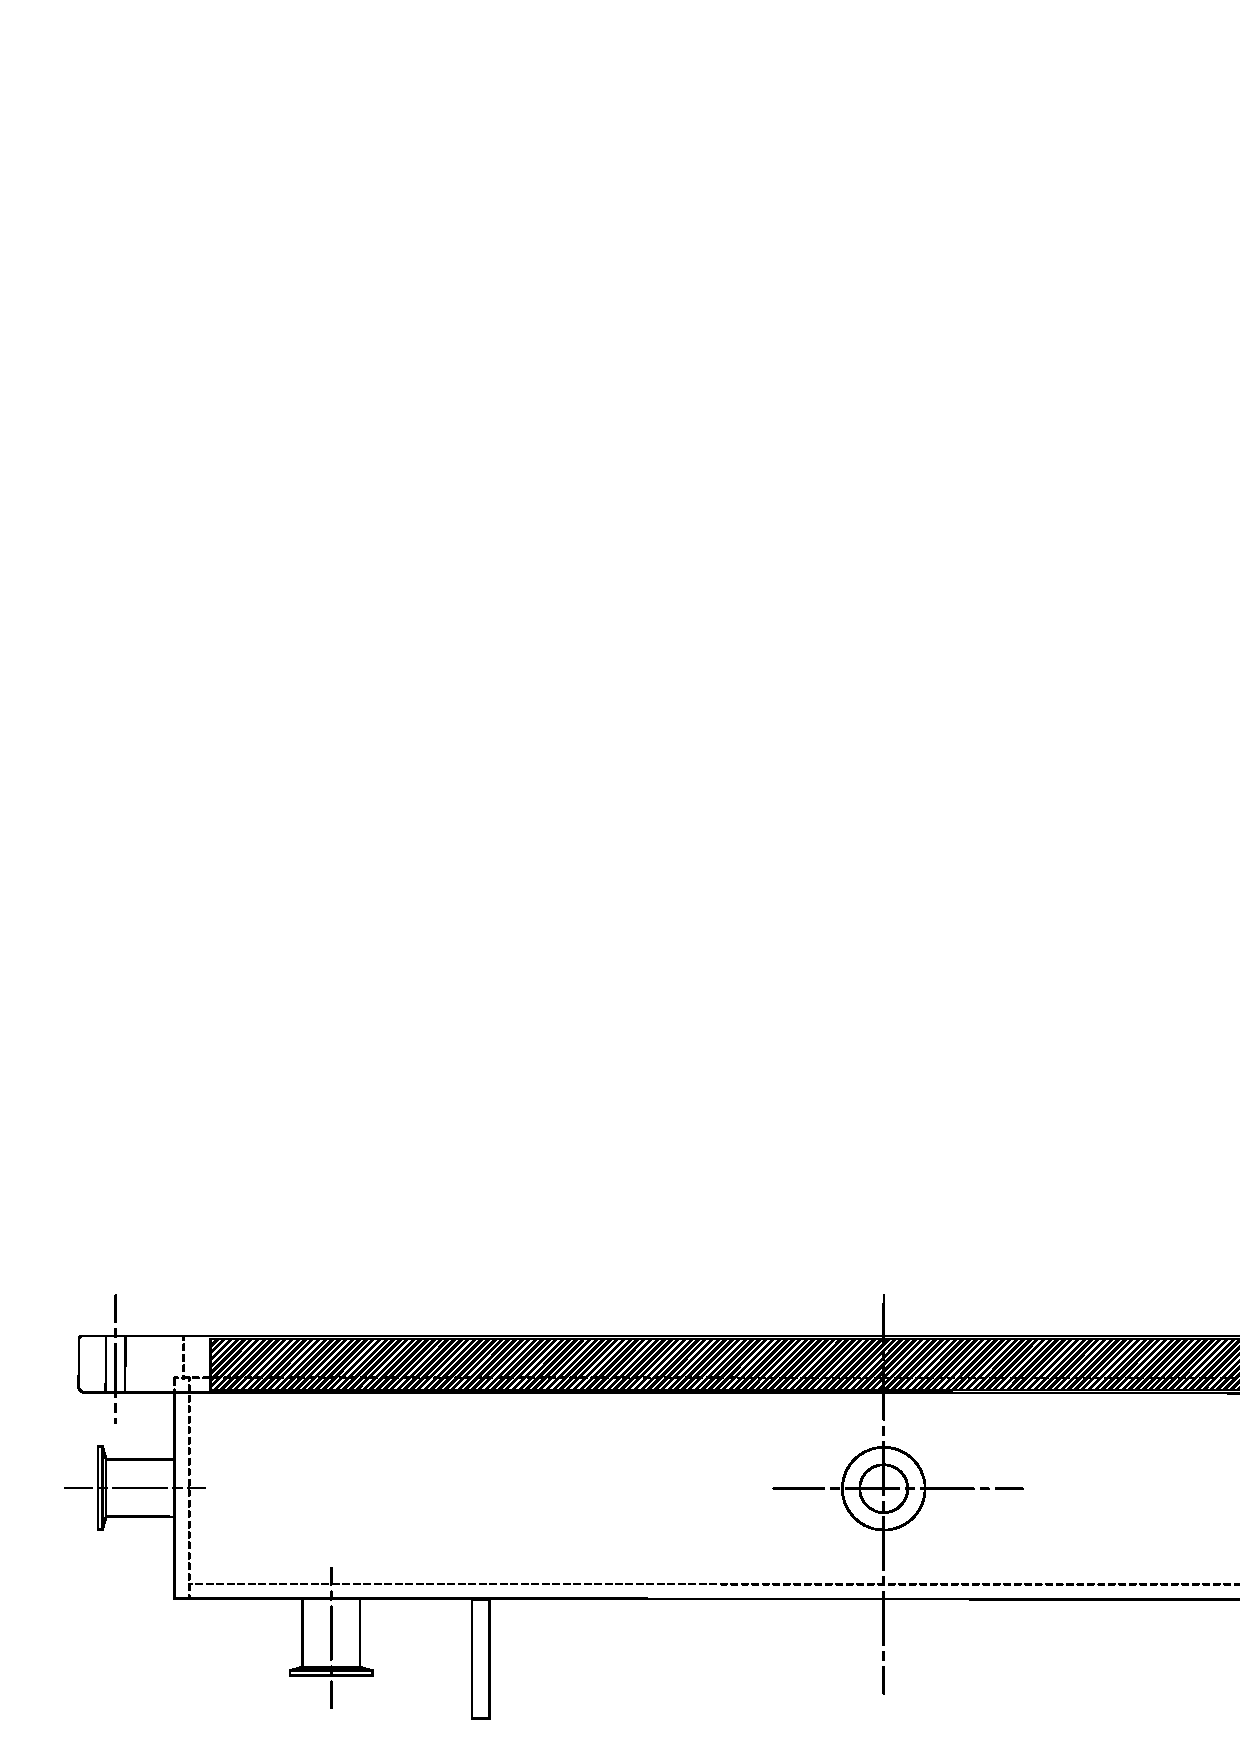
\includegraphics[width=6in]{figSOSwindow}
\caption{The SOS exit window and the vacuum test tank. \label{fig:sos_window}}
\end{figure}
\end{obsolete}


\infolevfour{
\paragraph{Window Material Testing}

Standard models used in predicting vacuum
window performance do not predict the actual performance of Kevlar laminate
fabrics accurately \cite{Mapes1993,Leonhardt,rllnl2}. Therefore, extensive tests of the
Mylar/Kevlar composite windows have been done and more are planned.
A summary of pressure
tests on windows composed of the custom laminated
fabric currently used in construction of all Hall~C vacuum windows is
given in Tables~\ref{tab:win_tst1} and \ref{tab:win_tst2}, below. Both vacuum and hydrostatic test 
tanks
are available for the HMS circular windows and for the SOS rectangular
window. Figure~\ref{fig:sos_window} shows a picture of the SOS vacuum
test tank.  The large round
HMS vacuum test tank uses the $8$ inch vacuum extension piece shown
earlier in Figure~\ref{fig:hms_window} (but removed from the spectrometer) with a $1.5$
inch thick aluminum blanking flange. For hydrostatic testing, windows (both
round and rectangular) are mounted directly on
blanking flanges with appropriate water fittings installed.

\begin{figure}
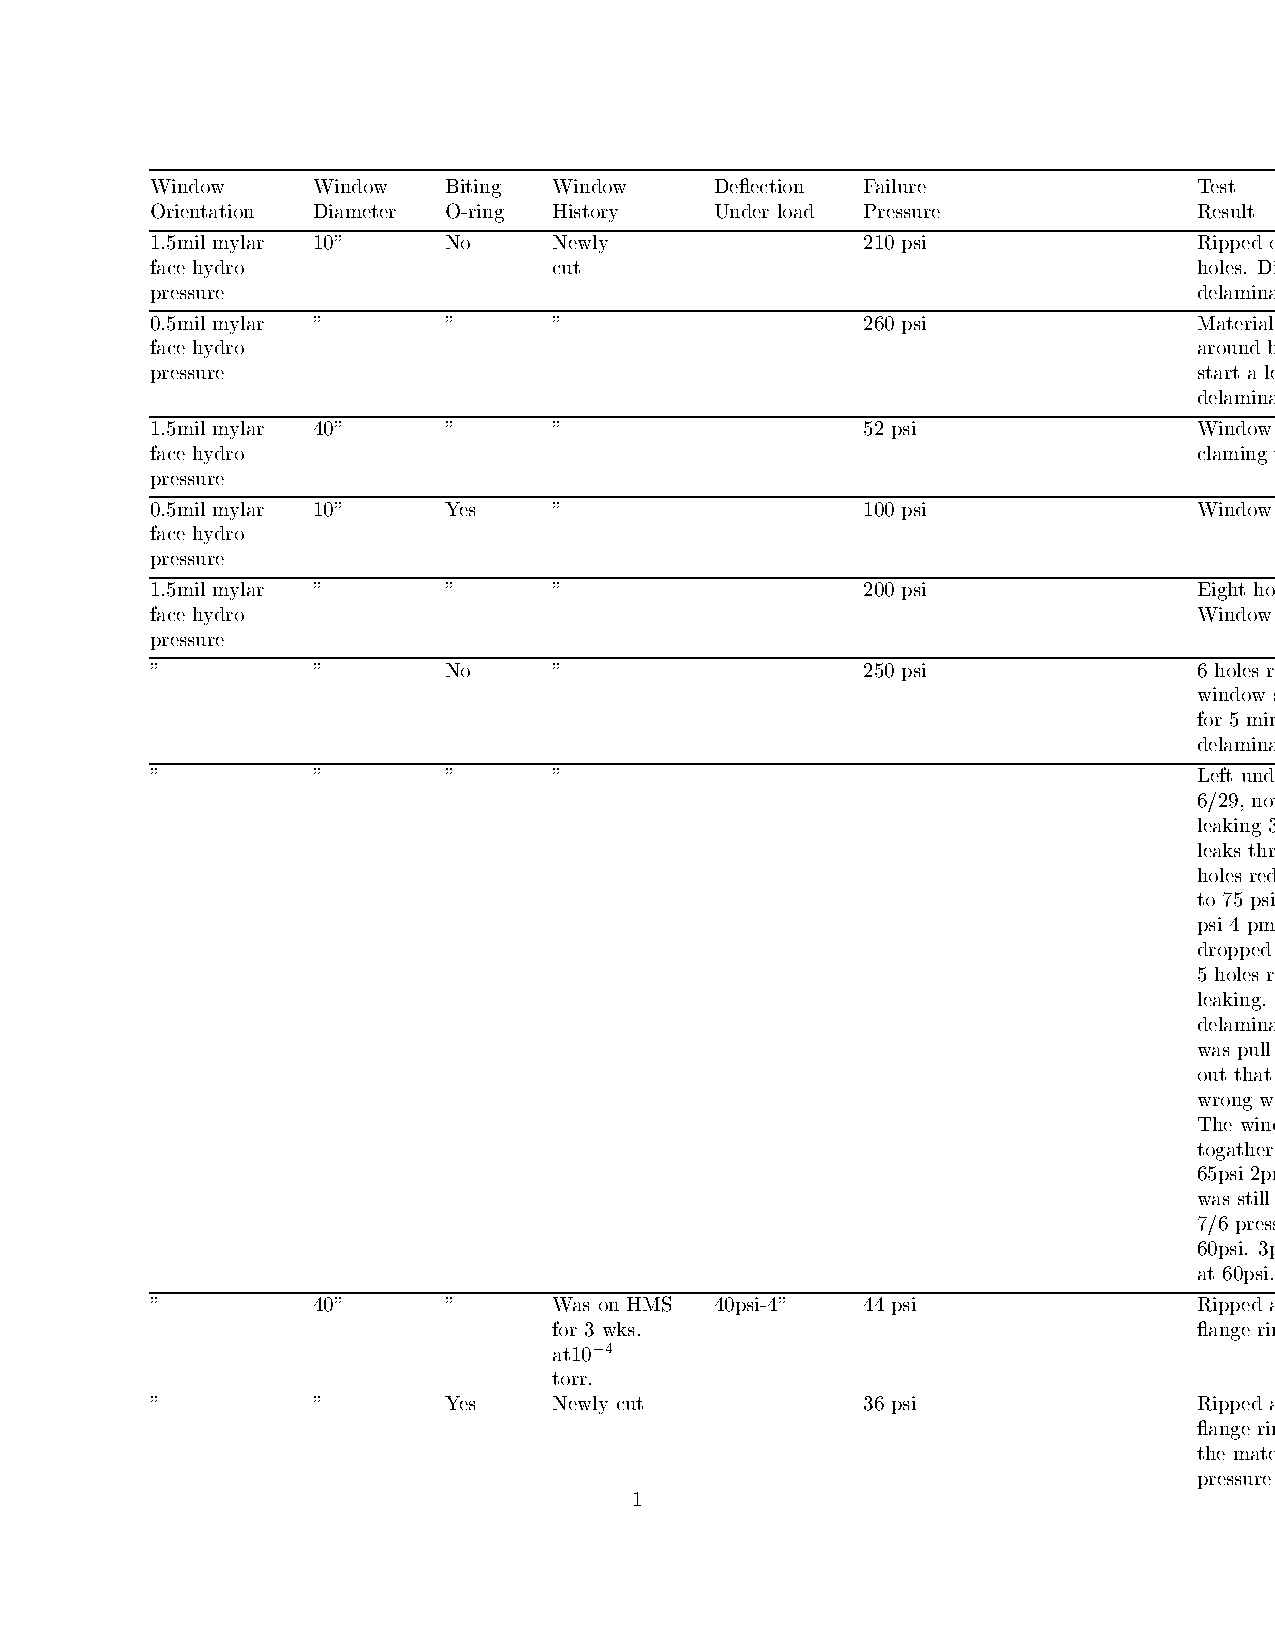
\includegraphics[height=7.5in]{vacuum}
\caption{Tests on the Hall~C Vacuum Windows (1 of 2) \label{tab:win_tst1}} 
\end{figure}
\clearpage

\begin{figure}
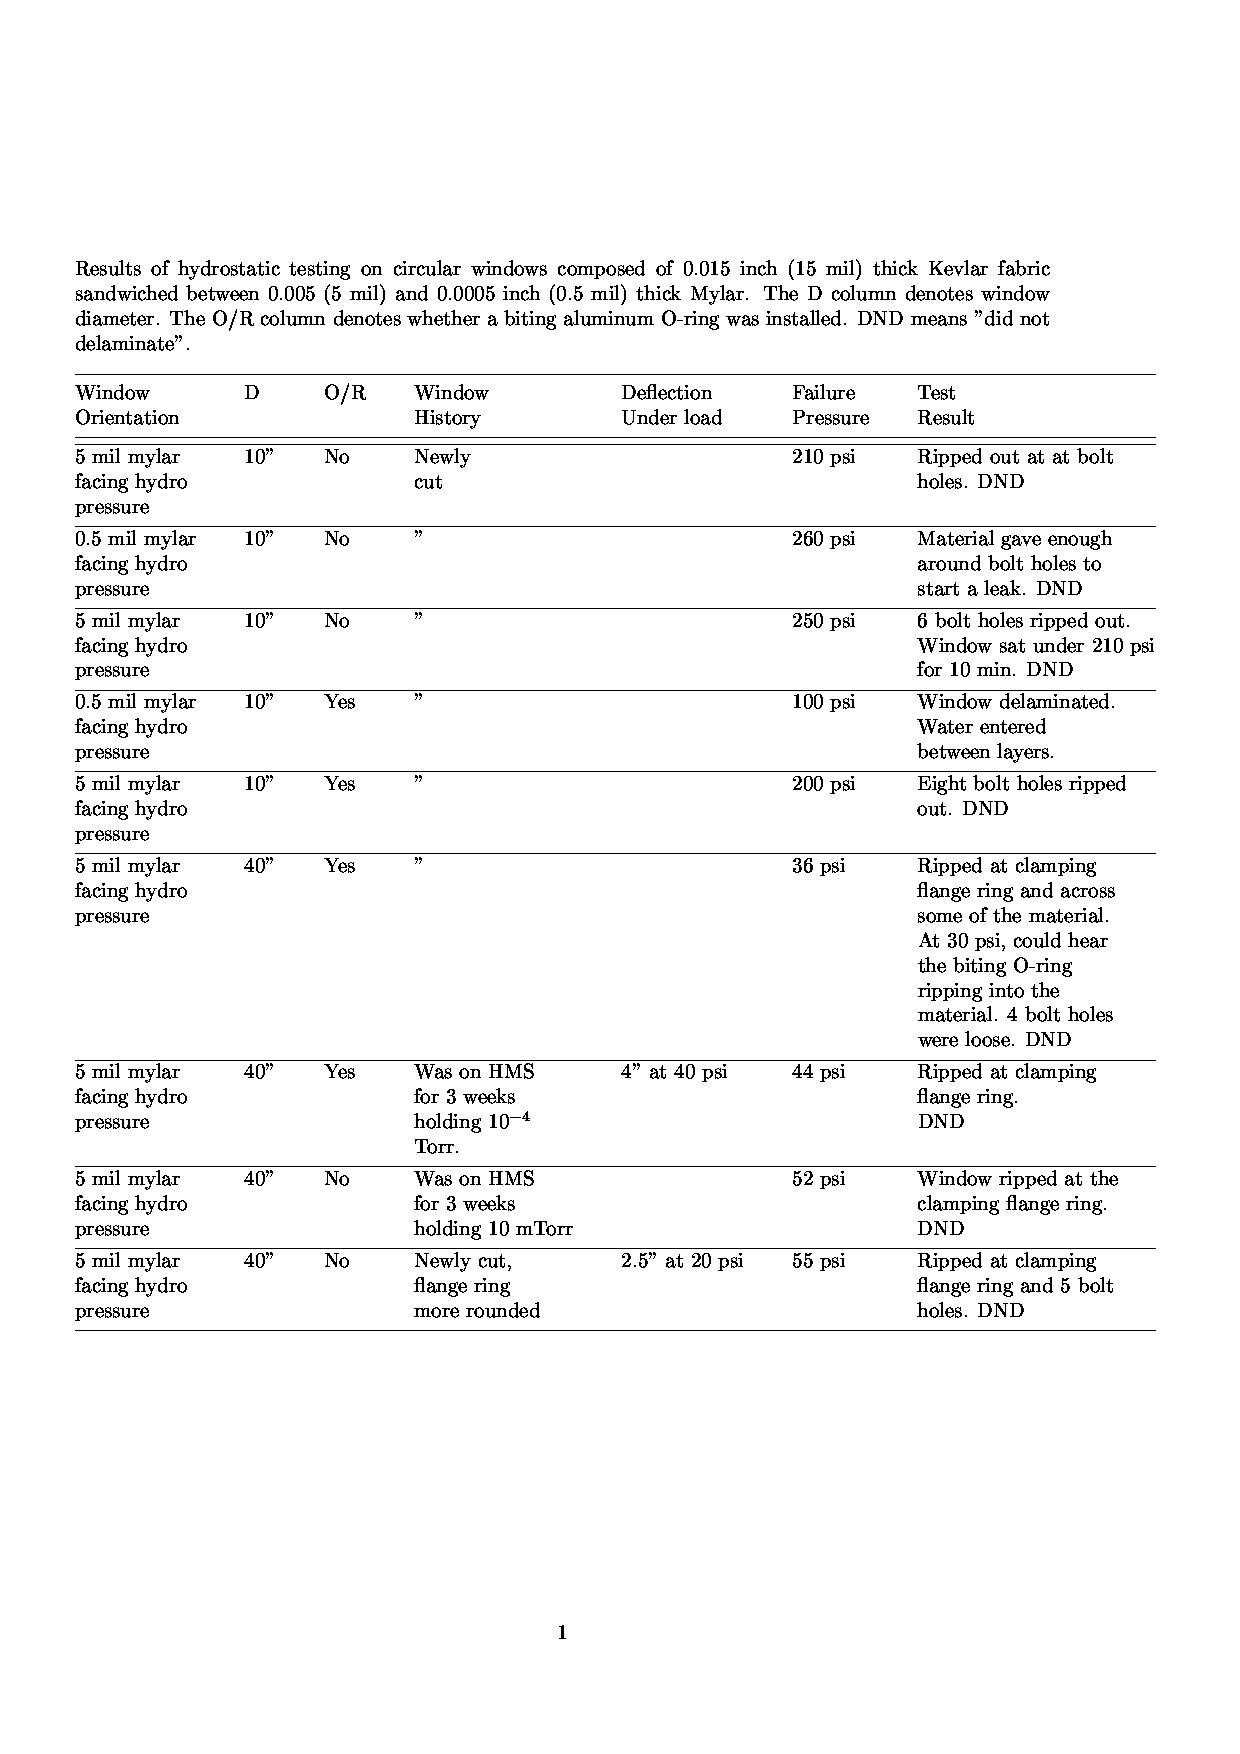
\includegraphics[height=7.5in]{vacuumc}
\caption{Tests on the Hall~C Vacuum Windows (2 of 2) \label{tab:win_tst2}}
\end{figure}
\clearpage

The tests show that the large HMS exit window does not begin to leak until
the pressure on it reaches over $3$ atmospheres. The small HMS window
did not begin to leak until over $14$ atmospheres of pressure was applied.
This is consistent with the load being transferred to
the outer circumference, the circumference of the small circle being four
times smaller than that of the large circle. The large rectangular SOS windows
began to leak at around 10 atmospheres. It may be possible to construct thinner
SOS vacuum windows for improved spectrometer resolution if required.

In addition to determining the absolute failure
pressure of the windows, a major goal of the testing effort was to
observe the failure modes of the
window material and flange design. The large windows failed by
ripping around the opening perimeter. The flange ring was then
rounded more and
a better result was obtained. It may be possible to further round the
flange if future tests indicate this to be necessary or advantageous.
The small windows failed by ripping out at the bolt holes.

Another question the tests in Table~\ref{tab:win_tst1} were designed to
answer was if
a biting aluminum clamping O-ring was necessary or advantageous. It was found
that windows with aluminum clamping rings failed at lower pressures than
windows without aluminum rings. The aluminum tended to tear the Mylar, allowing
leaking and uneven stress. The only window which delaminated had water between
the Mylar and Kevlar which leaked in through a tear in the
Mylar caused by the aluminum ring.

In conjunction with outlined full-size window testing, small samples
were subjected to stress and tensile analysis using strain gauge
instrumentation.  Through this work, it was found that the composite
window material maintained the Young's Modules of Kevlar, and had the
same ultinate failure load as Kevlar pieces of the same size.
Further, it was determined that the failure tears were along a
45$^{\circ}$ angle to the woven fibers, consistent with observations
of the rips in the destructively-tested full-size windows.  

In addition to the above testing efforts, two large round HMS exit windows
composed of the custom laminate material were ``knife" tested. The windows
were installed on the vacuum test tank and placed under vacuum. They were then
cut by a blade at the end of a long pole (so as to protect the personnel
testing the window from the results of a catastrophic failure). The window
did not rip any further than the cut and the
material did not delaminate. No evidence for catastrophic failure
was observed in either of these tests.

Although more long term reliability testing is necessary (see below),
results have so far been favorable.
Windows previously used on the HMS spectrometer are routinely hydro
tested to failure after biannual removeable and found to
hold up as well as freshly made windows (see, for example
Table~\ref{tab:win_tst1}).  Windows which have undergone multiple cycles fail at nearly the same pressure as uncycled
windows (see, for example, Table~\ref{tab:win_tst2}). A small round window did not fail after
being left pressurized for
a week at $65$ psi. (this test is not entered in the tables).
Entrance and exit windows composed of the Mylar/Kevlar laminate
material here described have held vacuum on the Hall C
spectrometer effectively and safely for over three years.


\paragraph{Vacuum Window Fabrication and Installation Procedure}

This procedure must be followed for installing any Hall~C spectrometer
vacuum window. One of the responsible personnel must be present during
all steps of fabrication and installation.
Although the procedure below is specifically for
the HMS large window, it is the same for the small HMS and for both SOS windows,
except as noted.
\begin{enumerate}
\item{Place window material, thin Mylar side down,
on a large flat, extremely clean, surface (such as
the marble table in EEL 126 after being washed).}

\item{Place window flange ring (also freshly cleaned) on top of material
and trace outer
circle (or rectangle for SOS) and bolt holes with transparency marking
pen.}

\item{Remove flange ring and cut out circle using Kevlar cutting 
shears.}

\item{Cut out bolt holes using appropriate (custom-made) drill press tool.
For the larger windows, this is a two person job as one is needed to hold the
material up so that it can't be nicked by the side of the drill press table
while the other concentrates on cutting the holes.}

\item{Clean the aluminum flange ring thoroughly and wipe with isopropyl
alcohol. For all but the HMS exit window, the flange ring and
window should be brought to the hall.  For the HMS exit window,
continue as outlined below from step 6 on.  For all other windows,
install flange ring and window unit to spectrometer vacuum flange
using standard O-ring vacuum seal practice (i.e. clean all surfaces
thoroughly with alcohol, apply vacuum grease, tighten in star pattern,
etc.)  All bolts should be torqued to 50 ft-lbs (40 ft-lbs for the
SOS exit window).  There must be a correctly tightened bolt in every
bolt hole.  Continue to step 17.}

\item{{\sl (HMS exit window)} Clean Viton O-ring with isopropyl alcohol and apply vacuum
grease as is standard for vacuum connections.}

\item{{\sl (HMS exit window)}Place Viton ring on HMS vacuum extension piece, composite
window over ring, and aluminum flange (clamping) ring over window.   Bolt together at four corners.}

\item{{\sl (HMS exit window)}Place and tighten bolts in a star pattern as appropriate for
standard O-ring vacuum seals.}

\item{{\sl (HMS exit window)}All bolts should be torqued to 50 ft-lbs (40 ft-lbs for the SOS
exit window).}

\item{{\sl (HMS exit window)}Using standard O-ring seal technique, mount other side of
vacuum extension piece on aluminum blanking flange.}

\item{{\sl (HMS exit window)}Using a transparency marker, trace the flange circle onto the
Mylar/Kevlar window.}

\item{{\sl (HMS exit window)}Begin vacuum pumping on extension
piece.} 

\item{{\sl (HMS exit window)}Note any creep of traced ring and window
deflection.  Check window for visual abnormalities or imperfections.}

\item{{\sl (HMS exit window)}Leave under vacuum for at least 1 hour.
Repeat step 13.}

\item{{\sl (HMS exit window)}Bring vacuum extension piece back to
atmospheric pressure and remove blanking flange.}

\item{{\sl (HMS exit window)}Being extremely careful not to touch the
Mylar/Kevlar window, install extension piece on HMS spectrometer in
hut using standard O-ring vacuum practice.}

\item{Clear detector hut and pivot area for initial pump down. Do not
allow entry for anyone other than the above named personnel to
these areas until a vacuum of at least 50 mTorr is achieved.}

\item{Begin vacuum pumping.}

\item{One of the above named personnel should check and note the
window deflections, recheck bolt torques, and generally look for
irregularities in the window deflections, before allowing
general entry to the detector
hut or pivot areas. That person should wear ear protection at all times while
near windows. Bolts should be retorqued if necessary.}

\item{Place a clearly visible tag near the vacuum window indicating
date of installation, estimated date of removal, and names and phone
numbers of contact personnel.}

\item{Recheck bolt torque, vacuum, and window deflection
again a couple of hours later (again, this should be done by
qualified personnel only, wearing hearing
protection). Retorque bolts if necessary.
If the window deflection has increased more than 3/4 inch, begin the entire
process again with a new window.}

\item{The windows should be changed as close to every 6 months as
reasonable given experiment run scheduling considerations. It is not
necessary to stop a run to change the windows, but they should be changed
as soon as possible thereafter.}

\end{enumerate}
} %infolevfour

%\paragraph{Safety Procedure for Working Near Vacuum Windows}

%Before entering the detector huts or pivot area, all personnel should check
%the spectrometer vacuum gauges. The HMS gauge is located under and near the Q3
%quadrupole. The SOS gauge hangs from the carriage beneath the quadrupole.
%Both gauges are monitored by video cameras and may be viewed
%in the counting house.
%If the spectrometers are under vacuum, the following procedure should be used.
%
%\begin{enumerate}
%\item{Before entering detector hut or pivot area, put on hearing
%protection. It is recommended that nobody should be
%closer than 3 feet from the windows without ear protection and that only
%those personnel who need to approach the windows be in their immediate
%vicinity.}
%
%\item{If entering HMS detector hut, close aluminum
%shutter over vacuum window before entering.}
%
%
%\item{If entering pivot area, check both spectrometer windows visually
%(from a distance greater than 3 feet if possible) for obvious wrinkles or
%discoloration. If any are observed, vacate area and
%contact one of the above named personnel. Never touch the vacuum 
%windows.}
%
%\item{Use careful judgement if it is necessary to work near the vacuum
%windows. Do not place objects so that they may fall on the windows, 
%etc.}
%
%\item{Do not work near the windows any longer than is absolutely
%necessary.}
%
%\item{Open aluminum
%HMS exit shutter only when all personnel have left the detector
%hut.}
%\end{enumerate}
%
%\paragraph{Vacuum Window Safety Summary}
%
%Catastrophic window failure would generate a significant shock wave as air
%rushed to fill the evacuated volume. It would make a loud noise which could
%damage the hearing of anyone standing close at hand at the time of failure.
%There are several indicators that something is wrong with the vacuum. If
%any of the following are observed, qualified personnel should be contacted
%and no one should approach the windows until one of those personnel have
%deemed it safe:
%
%
%
%\begin{enumerate}
%
%\item{Visual defects, particularly wrinkles, discoloration, or
%uneven fiber stress.}
%
%
%
%\item{Date of removal on tag near spectrometer window indicates
%a date near or after current date.}
%
%
%\item{Vacuum gauges indicating a loss of vacuum
%$\ge 1$ mTorr.}
%
%\item{HMS shutter malfunction (troubles opening or closing).}
%
%\item{The pen-traced ring drawn onto thae window perimeter moving away
%from the perimeter.}
%
%\item{Bolt torque not remaining at installed value
%(only qualified personnel should check for this).}
%
%\item{Deflection increasing above installed value
%(only qualified personnel should check for this).}
%\end{enumerate}
%





\section{Magnets and Power Supplies}

The HMS and SHMS magnets are all
superconducting and hence their coils must be maintained at
cryogenic temperatures during operations. The LHe required by the magnets
is supplied by the End Station Refrigerator, ESR.

All the spectrometer cryogenic services are supplied through the overhead
cryogenic lines. The distribution network begins at the distribution
box over the pivot. This box is connected to the rest of the network via the
flexible transfer lines over the pivot. The network is adjacent to
the upstairs catwalk of the HMS.

Cryogenic information about each magnet is available on the control
screens located in the Hall~C counting house.
\begin{obsolete}
These are located on the first deck
of the shield house by the ``pasta fork" at the rear of the spectrometer.
Normally during run periods the control screens are sent upstairs to the
Hall~C counting house and information on all the HMS magnets is available
on the HMS control screen located in the center of the main console.
The control of all magnets is described in a following Subsection.
\end{obsolete}

The power supplies for the magnets are located on the carriage
adjacent to the magnets. The supplies are all water cooled and
the water flow rate to the supplies can be seen on the water flow
meter located near the electronics boxes on the floor near the pivot.
Under normal conditions the meter should read
approximately 33 $\%$. This meter views the flow for all the HMS power supplies
(dipole and quads) and a reading of 33 $\%$ corresponds to approximately
20 gallons per minute through the combination of supplies (they are supplied
in parallel).

The front panels of the power supplies are interlocked. Under
no circumstances should the front panel of any supply be opened by anyone other
than authorized personnel. There is a keyed electrical interlock
located in the Hall~C counting house main console to prevent the
power supplies from being energized at inappropriate times.
Personnel listed in the relevant section of the ESAD for the Hall C
Base Equipment maintain a copy
of the key.

When the supplies are energized there are flashing red lights placed at
several locations on the HMS carriage to alert personnel to the magnet
status. There are also signs posted listing the dangers of high magnetic
fields.

The control interfaces for the power supplies are available in the 
Hall~C counting house on the HMS and SHMS control screens.

\paragraph{Personnel}
In the event that any problems arise during operations of the magnets
qualified personnel should be notified. This includes any prolonged
or serious problem with the source of magnet cryogens (the ESR).
In the weekend and after hours there
will be a designated individual on call for magnet services. Any member of
the Hall~C engineering group is qualified to deal with unusual magnet situations
but in the event of serious problems the chief cryo/mechanical engineer (Paul
Brindza) should be contacted.


\subsection{Quadrupole Magnets and Cryogenic Procedures}

\paragraph{Quadrupole Magnets}
The quadrupoles determine the transverse focusing properties of the spectrometer
and to a large extent its acceptance.

All three quadrupoles for the HMS spectrometer are cold iron superconducting
magnets. The soft iron around the superconducting coil enhances the field at
the coil center and reduces stray fields.
The basic parameters for the first quadrupole, Q1, are an effective (actual)
length of 1.89 (2.34) meter and an inner pole radius of
25.0 centimeter. \cite{bi:yan1}
The vacuum vessel
inner radius for Q1 is 20.05 cm. To achieve the lowest possible angle
setting of the HMS spectrometer (with respect to the beam line), Q1 is
made asymmetrical, and is elongated in the vertical direction. For the same
reason a notch in the outer mantle of the Q1 cryo vessel is made, such
that the incident electron beam passes through this notch when the
HMS spectrometer is at its smallest angle of 12.5 degrees.
The other two quadrupoles, Q2 and Q3, are essentially identical with an
effective (actual) length of about 2.10 (2.60) meter and an inner pole radius
of 35.0 centimeter. For these quadrupoles the vacuum vessel inner radius
amounts to 30.0 centimeter.

The maximum operating currents (assuming a 4 GeV/c momentum particle) for the
quadrupoles are about 580 A, 440 A, and 220 A, for Q1, Q2, and Q3, respectively.
To establish a correct focusing onto the detector plane with
the quadrupole triplet we may want to cycle the quadrupoles to about 20\% higher
current values, rendering maximum currents of 700 A, 530 A, and 270 A,
respectively. This will render pole field values of 1.25, 1.30, and 0.65 T,
respectively.
The energy stored in the quadrupole fields is sufficient to cause an
unrecoverable quench if all the energy stored is dumped into the
magnets. \cite{bi:hms1}
Therefore a quench protection circuit is incorporated. However, a quench
can only happen if the cryomagnets have a helium level below the coil during
operation.

The operating current to the quadrupole coils is provided by three
Danfysik System 8000 power supplies, which can operate up to 1250 A current
and 5 V voltage. The power supplies are cooled with a combined maximum 
water flow of 45 liters per minute.

In addition to the main quadrupole windings, all quadrupoles have multipole
windings. To further optimize focusing properties of the HMS magnet system
we may operate some of these multipole trim coils
\cite{bi:yan2}.
The operating current for these multipole
corrections is small (the multipole corrections are typically less than
2\% of the main quadrupole field), of order 50 A, and are provided by
three HP power supplies. These power supplies can operate up to 100 A current
and 5 V voltage.


\paragraph{Cryogenic Procedures}

\paragraph {First Time Startup Check List.}

See Oxford Instruments User manual for startup check list. \cite{bi:oxf1}

\newpage
\paragraph {Routine Startup Check List Before Energizing Magnets.}

A routine checkout of the quadrupoles by a Hall C Eng. Staff only should include as a minimum
the following:  Magnetic Materials Checks; Vacuum Checks; Cryogenics
and Valve Checks; Electrical and Main Power Supply Checks; and
Computer Control Checks.  A separate check list is included for shift
leaders.  

\subparagraph{Magnetic Materials Checks:}

\begin{itemize}
\item[{[~~~~]}]{Perform a walk around of magnet looking for loose magnetic
materials that could be attracted to the magnet during operation.}
\item[{[~~~~]}]{Check for sensitive electronic equipment that could be
effected or damaged by magnetic fields.}
\item[{[~~~~]}]{Advise any personal near HMS of magnet operations.}
\item[{[~~~~]}]{Ensure that magnetic field signs are posted near magnets
and HMS personnel ladders.}
\end{itemize}


\subparagraph{Vacuum Checks:}

\begin{itemize}
\item[{[~~~~]}]{Verify vacuum via readback on helium page.  (Vac=.25x10${^-6}$ Bar).}
\item[{[~~~~]}]{Check that Helium and Nitrogen Supply valves are at nominal
positions.  Excessive supply valve openings could indicted a higher heat
leak to the magnet cyrogens.}
\item[{[~~~~]}]{Check for condensation and freezing on Outer Vacuum
Chamber (O.V.C.).}
\end{itemize}

\subparagraph{Cryogenics and Valve Checks:}

\noindent On Magnet:

\begin{itemize}
\item[{[~~~~]}]{Visual inspection of magnet cryostat for condensation or frosting.}
\item[{[~~~~]}]{Visual inspection of U-Tubes (connecting distribution can to
magnets) for condensation of frosting.}
\item[{[~~~~]}]{Visual inspection of magnet turret top plate for indications
of any icing other then N2 exhaust pipe.}
\item[{[~~~~]}]{Audible check for any noise indicating a gas leak within main
leads cover housing on top of turret.}
\item[{[~~~~]}]{Check that heater tape is working on top neck of turret can.}
\item[{[~~~~]}]{Visually check all valve actuators for cable connections, LVDT
connections, relative stem position and motor operation.}
\item[{[~~~~]}]{Visual and audible inspection inside distribution box
(located on side of turret can) for leaks.}
\item[{[~~~~]}]{Inspection of lead flow valves for proper operation and position.}
\item[{[~~~~]}]{Check that heaters are set to $\sim$40 C and are working inside
distribution box.}
\item[{[~~~~]}]{Ensure that all manual valves are in correct position for normal
operation.  Helium lead flow/neck flow exhaust valve is to be open. Helium
Cooldown/Warm-up valve is to be closed.}
\end{itemize}

\noindent At Control Rack:

\begin{itemize}
\item[{[~~~~]}]{Verify that helium meter and N2 meter are on and indicating
proper liquid levels. Verify that helium meter and monitor display on helium
page are in close agreement.  (Typically the helium meter reads 4 to 5 percent
higher than monitor.)}
\item[{[~~~~]}]{Verify that nitrogen meter and monitor display on nitrogen
page agree with each other.}
\item[{[~~~~]}]{Check temperatures on monitor temperature screen.}
\item[{[~~~~]}]{Check temperatures on monitor helium screen. (4.4-4.7 K)}
\item[{[~~~~]}]{Check temperatures on monitor nitrogen screen. (77.- 80 K)}
\item[{[~~~~]}]{Check helium pressure on monitor reads about 1.34 Bar.}
\item[{[~~~~]}]{Check neck flow and current lead flows are reading near 10
L/min. with no current.  The current lead flow valves position should read
near 10\% open.}
\item[{[~~~~]}]{Make sure that PSU is disabled, Type on command line
PSU:SETCUR:1023.0.  Verify that lead flow readings increase to around 24
L/min. and that valve position readings increase.}
\item[{[~~~~]}]{Type on command line PSU:SETCUR:0.0. Verify that lead flow
valves return to previous valves (10L/min. at 10\% open).}
\item[{[~~~~]}]{Check the following valves for control and read back by opening
and closing the valve by 5\%(max.).}

\begin{center}
  \begin{tabular}{ll}
Valve 8	& Helium Cold Supply Top Fill		\\
Valve 6	& Helium Cold Supple Bottom Fill	\\
Valve 13& Helium Cold Return			\\
	& (Verify that Helium Pressure changes  \\
        &  with valve opening and closing)      \\
Valve 3	& LN$_2$ Supply Top Fill		\\
  \end{tabular}
\end{center}
\item[{[~~~~]}]{All other valves should be at a hard set -i.e. -6\% to
-3\% except the nitrogen check valve, \#19, which should read OPEN.}
\item[{[~~~~]}]{Go to trend page and verify that nitrogen and helium levels
have been maintained at proper levels for the last 24
hours.  (Helium level 75\%, Nitrogen Level 70\% to 80\%).}
\end{itemize}


At a remote terminal logged into a cdaq2 account:

\begin{itemize}
\item[{[~~~~]}]{Check HMS data logging program for the following:

Properly logging HMS and CHL data.

HMS transfer line temperature probes are correct.  (Displayed as
Carriage Temperatures).}
\begin{center}
  \begin{tabular}{lll}
T1	& 5.4 to 5.5 K	& Helium Supply Temp. 1	\\
T2	& 5.5 to 5.8 K	& Helium Supply Temp. 2	\\
T3	& 78 to 180 K	& Nitrogen  trace line.	\\
T4	& 4.4 to 4.6 K	& Dipole helium return.	\\
T5	& 5.4 to 5.6 K	& Dipole helium inlet.	\\
  \end{tabular}
\end{center}
\item[{[~~~~]}]{Check that CHL data is reasonable.}
\begin{center}
  \begin{tabular}{lll}
CFI1139 & 5.0 to 10.0 g/s & He supply Flow \\
CPI671T & 2.4 to 2.8 atm & He supply Pressure \\
CPI9521 & 1.14 to 1.17 atm & He return Pressure \\
CTD671T & 5.2 to 5.6 K & He supply Temp. 1 \\
CTD9521 & 5.3 to 5.7 K & He supply Temp. 2 \\
\end{tabular}
\end{center}
\item[{[~~~~]}]{Check with CHL about their present and future status.}
\end{itemize}


\subparagraph{Electrical and Main Power Supply Checks:}

\begin{itemize}
\item[{[~~~~]}]{480V Main circuit Breaker:  should be locked OFF
before opening Main Power Supply cabinet doors.}
\item[{[~~~~]}]{Individual 208V magnet circuit breakers are in the on
position.  (Located within service lug near center pivot.
Q1:\hskip0.3in ,Q2:\hskip0.3in ,Q3:\hskip0.3in ).}
\item[{[~~~~]}]{Check for Magnet short to ground. Record resistance measurements.}
\item[{[~~~~]}]{Visual inspection of main current leads connection inside of
Main Power Supply. Check for loose connections.}
\item[{[~~~~]}]{Control computer up and running.}
\item[{[~~~~]}]{Quench Detector powered and no interlocks.}
\item[{[~~~~]}]{Interface Unit powered and no interlocks.}
\item[{[~~~~]}]{Control rack power supplies operating  (Three power supplies
located at bottom of rack).}
\item[{[~~~~]}]{Energy dump rack powered and interlock cable connected. Test
Energy dump switch by unplugging interlock cable. Reconnect interlock cable
and reset dump switch. Clear interlocks at control rack.}
\item[{[~~~~]}]{Repeat energy dump test by unplugging power cord to rack.
Clear interlocks.}
\item[{[~~~~]}]{UPS power verified within control rack.}
\item[{[~~~~]}]{Check LCW supply and return pressures as well as flow rate.
[Near pivot].}
\item[{[~~~~]}]{Ensure that cooling water is turned on to power supply.}
\item[{[~~~~]}]{Check for water leaks within power supply unit.}
\item[{[~~~~]}]{Close all doors and cabinets.}
\item[{[~~~~]}]{Turn on 480V main circuit breaker.}
\item[{[~~~~]}]{Ensure that the power enable switch (located in Hall~C
counting room) is enable.}
\item[{[~~~~]}]{Turn on power supply switch.}
\item[{[~~~~]}]{Check all interlocks displayed on power supply led display.
Clear interlocks via front panel reset button on power supply unit.}
\item[{[~~~~]}]{Turn off water supply to power supply. Check that water
flow interlock comes on. Turn water back on and reset interlock.}
\item[{[~~~~]}]{Open front door of PSU. Check door interlock. Secure door and
reset interlock.}
\item[{[~~~~]}]{Test Panic button on front of PSU. Reset.}
\end{itemize}

\subparagraph{Computer Control Checks:}

\begin{itemize}
\item[{[~~~~]}]{Clean PC's Dust filter.}
\item[{[~~~~]}]{Go to Interlock screen. Verify and clear any interlocks.}
\item[{[~~~~]}]{Go to Power supply screen. Enable Power supply control by
typing in command line ``Mode:Normal".}
\item[{[~~~~]}]{Type on command line ``PSU:Remote".}
\item[{[~~~~]}]{Type on command line ``PSU:Reset".}
\item[{[~~~~]}]{Type on command line ``PSU:On".}
\item[{[~~~~]}]{Observe if magnet ``ON" lights (magenta flashing lights) are
activated on HMS carriage.}
\item[{[~~~~]}]{Go to Coil Monitor screen.}
\item[{[~~~~]}]{Type on command line ``Psu:setcur:100.0"}
\item[{[~~~~]}]{Observe coil voltages and current lead voltage readback. Note
any unusual behavior.}
\item[{[~~~~]}]{Activate the shutdown icon on power supply screen.}
\item[{[~~~~]}]{Clear interlocks and turn PSU back on.}
\item[{[~~~~]}]{Test polarity reversing switching.}
\item[{[~~~~]}]{Type on command line ``PSU:standby".}
\item[{[~~~~]}]{Type on command line ``mode:standby".}
\item[{[~~~~]}]{Pass control of magnet up to counting house.}
\item[{[~~~~]}]{Verify safe operation of control system from counting house.}
\end{itemize}

\vspace{0.5in}
\hspace*{3.5in}{\underline{~~~~~~~~~~~~~~~~~~~~~~~~~~~~~~~~~}}
\newline
\hspace*{3.5in}{Signature~~~~~~~~~~~~Date}


\newpage
\paragraph{Long Term Shutdown - Restart Check List:}

A long term shutdown shall be defined if any of the following
conditions is satisfied: a period of time that exceeds 2 months without
having energized the magnets, after a magnet has been warmed to room
temperature and then re-cooled to operating temperatures or after a
replacement/repair of a major piece of equipment directly related to the
operation of the magnet, such as energy dump, main power supply, quench
detector, electronic interface unit, or control PC.  The check out list for
operating the magnets after a long term shut down shall include:

\begin{itemize}
\item[{[~~~~]}] {To be performed by approved Hall C engineering staff.}
\item[{[~~~~]}] {Off line test and confirmation of repaired or
replacement (R\&R) part (if warranted).}
\item[{[~~~~]}] {Test and verification of connections between R\&R
part and the control system.}
\item[{[~~~~]}] {Verification of all electrical and sensor
connections within control rack.}
\item[{[~~~~]}] {Perform a full interlock test.}
\item[{[~~~~]}] {Quench Detector threshold levels tested via the
quench detector test boards.}
\item[{[~~~~]}] {Perform the Routine Startup Check list.}
\item[{[~~~~]}] {Perform a full current ramp [200 amps steps] and
soak for one hour
at full current for each polarity. Record voltages for the coil, leads, and
the power supply output voltage. Ramp magnet down.}
\end{itemize}

\vspace{0.5in}
\hspace*{3.5in}{\underline{~~~~~~~~~~~~~~~~~~~~~~~~~~~~~~~~~}}
\newline
\hspace*{3.5in}{Signature~~~~~~~~~~~~Date}

\newpage
\paragraph{Annual Check List:}

On an annual basis a complete check out of the control system
shall be done. This should include at the least the following checks by a
qualified operator:

\begin{itemize}
\item[{[~~~~]}] {A complete test of interlocks and protection devices.~\cite{bi:oxf2,bi:danf}}
\end{itemize}

At the control rack test the following:

\begin{itemize}
\item[{[~~~~]}]{Watchdog.}
\item[{[~~~~]}]{He Neck flow.}
\item[{[~~~~]}]{He reservoir low.}
\item[{[~~~~]}]{He pressure high.}
\item[{[~~~~]}]{N2 pressure high.}
\item[{[~~~~]}]{CEBAF shutdown.}
\item[{[~~~~]}]{Trim Coil Quench.}
\item[{[~~~~]}]{Dump Switch open.}
\item[{[~~~~]}]{Current Lead overvoltage.}
\item[{[~~~~]}]{Main Coil overvoltage.}
\end{itemize}


At the power supply test:

\begin{itemize}
\item[{[~~~~]}]{Control Rack I/L.}
\item[{[~~~~]}]{Panic / Door I/L. (Panic switch)}
\item[{[~~~~]}]{Panic / Door I/L. (Door switch)}
\item[{[~~~~]}]{MPS waterflow.}
\item[{[~~~~]}]{MPS overtemp.}
\item[{[~~~~]}]{Phase Failure.}
\item[{[~~~~]}]{Reg. Module Failure.}
\item[{[~~~~]}]{Max. Current Set.}
\item[{[~~~~]}]{Transducer Fail.}
\item[{[~~~~]}]{Transistor Failure.}
\item[{[~~~~]}]{Fuse Failure.}
\end{itemize}

\begin{itemize}
\item[{[~~~~]}] {Quench detector threshold levels tested and values recorded.}
\item[{[~~~~]}] {Test of backup temperature probes and voltage taps.}
\item[{[~~~~]}] {Control PC performance checked out and recorded.}
\item[{[~~~~]}] {PC's ADC tested.}
\item[{[~~~~]}] {Verification of all electrical and sensor connections within control
 rack.}
\item[{[~~~~]}] {Inspection of power lead cables within power supply, energy dump
rack and along cable tray up to magnet connection.}
\item[{[~~~~]}] {Inspection of signal cables.}
\item[{[~~~~]}]  {Perform a full valve stroke of all cryogenic valves.}
\item[{[~~~~]}] {Check U-tubes vacuum.}
\item[{[~~~~]}] {Re-calibrate pressure gauges.}
\item[{[~~~~]}] {Inspection of Safety devices (rupture disk, relief valves, parallel
plates).}
\item[{[~~~~]}] {Backup check of O.V.C. vacuum via C.E.B.A.F.'s cold cathode gauges
and/or a RGA system.}
\item[{[~~~~]}] {Visual inspection of control rack's internal electrical components}
\item[{[~~~~]}] {Visual inspection of energy dump rack's internal electrical
components and connections.}
\item[{[~~~~]}] {Record energy dump's resistance.}
\item[{[~~~~]}] {Record power lead cables resistance.}
\item[{[~~~~]}] {Test trim coils.}
\end{itemize}
%\newpage
Perform Maintenance on main power supply as describe by Danfysik 
power supply (See Magnet Power Supply System 8000 section 5, page 77 to 78.).
\begin{itemize}
\item[{[~~~~]}] {Verify power supplies current limitation settings (front panel and
internal settings).}
\item[{[~~~~]}] {Check for short to ground. Record resistance measurements.}
\item[{[~~~~]}]  {Do a routine start check list.}
\item[{[~~~~]}] {Perform a slow discharge of magnet at full field. Record magnet
voltage vs time. Repeat with opposite polarity.}
\item[{[~~~~]}] {Perform a fast discharge of magnet at full field. Record magnet
voltage vs time. Repeat with opposite polarity.}
\item[{[~~~~]}]  {Clean and dust components.}
\end{itemize}

\vspace{0.5in}
\hspace*{3.5in}{\underline{~~~~~~~~~~~~~~~~~~~~~~~~~~~~~~~~~}}
\newline
\hspace*{3.5in}{Signature~~~~~~~~~~~~Date}

\newpage
\subsection{Dipole Magnet }

The dipole is the dispersive element in the system and 
determines the central momentum of the spectrometer.
The present operations envelope states that the supply may not be
operated at currents above 1300 Amps. This corresponds to a central
momentum of $\approx$4 GeV/c.

The dipole for the HMS spectrometer is a superconducting, cryostable magnet.
Its basic parameters are an effective length of 5.26 meter,
a bend radius of 12.06 meter, and a gap width of 42 cm.
Its actual size is 5.99 meter long, 2.75 meter wide, and 4.46 meter high.
It is configured to achieve a 25 degree bending angle for 4 GeV/c momentum
particles at a central field excitation of 1.11 T.
For the HMS dipole to reach 1.11 T the maximum operating current for the coil
amounts to 1300 A.

The dipole has been designed to achieve cryostability up to a field of 2 T,
and this property has been extensively tested up to a field of 1.11 T.
The cryostable coils are equipped with an energy removal circuit to cover
the possibility of an unrecoverable quench. \cite{bi:hms2}
However, this can only happen
if the helium level drops below the coil during operation.
The current to the coils will be provided by a Danfysik System 8000 power
supply, which can operate up to 3000 A current and 10 V voltage.
This power supply is located on the carriage beside the dipole, and
is cooled with a maximum water flow of 35 liters per minute.
The flow of the magnet cooling water is regulated by flow meters installed
on the floor of Hall~C. The total water flow needed to cool the 4 power
supplies for the HMS magnet system (dipole and quadrupoles) amounts
to 80 liters per minute, with a supply pressure of cooling water for
Hall~C of 250 psi.


\subsection{Operation of the HMS Magnets}

\paragraph{Introduction}

This is an abbreviated operating manual for the HMS superconducting
magnets specifically designed for Hall~C experimenters. It provides
instructions for setting currents, invoking NMR field regulation and
general system monitoring.  Curious readers are directed to the
references for more in depth operating instructions and other technical
manuals.

\vskip 0.2 true in
\begin{center}
\begin{tabular}{ll}
\multicolumn{2}{l}{\bf References}\\
\hline
\multicolumn{2}{l}{ELIN HMS Dipole operation manual}\\
Appendix 24 &  User Manual \\
Appendix ~5 &  Power Supply \\
Appendix ~6 &  NMR Tesla meter \\
Appendix ~7 &  NMR Field Regulation \\
Oxford HMS Quad & User Manual \\
Oxford HMS Quad & Technical Manual \\
TOSP & HMS Dipole \\
TOSP & HMS Quadrupole \\
HMS & SC Dipole Magnet Safety Review Vol. 1 and 2 \\
HMS & SC Quad Safety Review Vol. 1 and 2 
\end{tabular}
\end{center}

\paragraph{Magnet Currents}

The polarities of the currents in the HMS magnets are such that
Q2 and DIPOLE have the same sign as the charge of the particles
to be transmitted, Q1 and Q3 have the other sign.
To obtain the correct field settings for the HMS superconducting magnets
we use the following procedure:

\begin{itemize}
\item{To obtain the predicted current or field settings, run ``field" from
cdaqs1 or cdaqs2 when logged in as cdaq (at the moment
only the point-to-point tune is implemented). Look in the directory 
{\tt ~cdaq/FIELD for the latest version}}
\item{Use the ``setcurrent" values for the Quadrupoles.}
\item{Use the Field Setting Procedure for the Dipole. This will bring the
magnet to a field near but not equal to the desired field.}
\item{Turn field control on for the Dipole. The magnet will go to the
desired field.}
\item{Wait at least 7 minutes for the dipole magnet to settle.}
\end{itemize}

Up to this moment we have not witnessed any clear signature of hysteresis
effects for the dipole magnet. For the quadrupole magnets a small effect
on the field has been witnessed, but only for low currents (typically smaller
than 100 A). A procedure for setting the quadrupoles was developed
and shown to achieve a high
degree of reproducablility in setting the quads at low current.  The procedure
given here is taken from that procedure, but has not yet  been tested.\\
\textbf{The procedure:} 
\begin{enumerate}
  \item{On every change of polarity, take the magnet up to 950 Amps 
     (in the new polarity!), then down to zero before setting the
     current.} 
  \item{To set the current the first time after a polarity change 
     go up to 200 Amps higher than the desired current, 
     then down to the desired current.

     This means: to change the polarity and set the current go to 950 Amps,
     down to zero, back up to 950 Amps, and down to the desired setting.}
  \item{Subsequently:
  \begin{itemize}
     \item{Changes to lower currents can be made directly. 
        That is, just set the magnet for the lower current.}
     \item{For changes to higher current, first overshoot 
        by 200 Amps, then come back down to the desired current.}
  \end{itemize}}
\end{enumerate} 
This procedure is called \textbf{CYCLING
THE MAGNET}, and needs to be  followed for all three quadrupoles.

\begin{obsolete}
\paragraph{Magnet Selection}

The superconducting magnet keyboard and video signals are transmitted to
the Counting House via a switchable link.  The video is amplified and
the Counting House quality is as good as that in Hall~C.  The keyboard
commands are somewhat slower than the local keyboards but usually work
properly.  Occasionally junk commands (usually a string of dots) appear
in the quad dialogue box due to the switching.  The quads usually ignore
all bad commands.

\paragraph{Selecting a magnet}

\begin{center}
\begin{tabular}{lll}
\multicolumn{3}{c} {Sequence of keystrokes...How to select a magnet.}\\
\hline
        &Press and hold &``Num lock"	\\
        &Press and hold	&``minus (--)"	\\
        &Release	&``minus (--)"	\\
        &Release	&``Num lock"	\\
        &Press one of	&``A" for Q1	\\
        &  	&``B" for Q2	\\
        &		&``C" for Q3	\\
        &		&``D" for Dipole	\\
        &Press		&``Return"	\\
  \end{tabular}
\end{center}

\paragraph{Using the keyboard}

\begin{description}
\item{\bf 1~}\hskip0.1in The quadrupoles use only normal keyboard operations
such as
Alphanumeric keys, cursor keys, and return for selection.  The ``Esc"
(escape) key is also used for menu selection.  The ``Home" key is used to
move from the upper screen to the lower screen.  ({\bf Note:} Num Lock
must not be on to use home key on Num pad).
\item{\bf 2~}\hskip0.1in The dipole keyboard has a built in track ball that
is not
emulated in the Counting House.  You must use the cursor keys and then
type ``exec" (execute) to make a selection, i.e. to plot a graph, select
from a screen menu or to access a valve control menu.  The dipole makes
extensive use of the ``f" keys and a menu is always on the bottom of the
screen.
\item{}\hskip0.3in {\bf Note:  F8 exits the program and saves the trend data}
\item{}\hskip0.3in The alpha numeric keys are used as usual although the PDS
(dipole interface) is built around ``point and click" so only an occasional
number entry is required.
\item{\bf 3~}\hskip0.1in Saving Data
\item{\bf 3.1~}\hskip0.1in The quad system saves data for up to 1 week
without operator
intervention. The data must be transferred to floppy disc to ensure
that it is not overwritten.
\item{}\hskip0.3in {\bf Note:} The quad (Paragon) system start command is
``CEBAF"
\medskip
\item{\bf 3.2~}\hskip0.1in The dipole does not automatically save data without
assistance from an operator.  The dipole has a fast ($\sim$ 2 hour)
buffer and a slow ($\sim$ 1 week) buffer.  The data is stored in 1
day/20 min subsets.  The data can be saved by typing
\end{description}

\begin{center}
  \begin{tabular}{cccc}
	&FREEZE/TR=0 	&	& (RETURN)	\\
	&		& and	&		\\
	&FREEZE/TR=1	&	& (RETURN)	\\
  \end{tabular}
\end{center}

\begin{description}
\item{}\hskip0.3in The data will also be saved by pressing the F8 key to
exit the
PDS program. You must type ``HMS" (return) at the DOS prompt to restart.
Saving the data is a good idea but exiting the program is not,
therefore exit (F8) only in desperation.
\item{\bf 4~}\hskip0.1in Rebooting
\item{}\hskip0.3in It is possible to perform a soft boot ``CTRL - ALT - DEL"
from the Counting House keyboard.  The remote system has a hard time
transmitting this, possibly because it is too slow.  Multiple tries are
occasionally necessary.  This should not be done except under desperate
circumstances.
An alternative method is via the reboot button located upstairs in
the counting room/data acquistion section.  Turn the knob to the
correct magnet then press and release the reboot button.

\item{}\hskip0.3in {\bf Note:If you need to restart the HMS control screen, the command to issue at the DOS
prompt is "HMS" (without the quotes).}


\end{description}
\end{obsolete}

\paragraph{Checking Cryogenics}

\begin{description}
\item{\bf 1}\hskip0.1in Routine checking
\item{}\hskip0.3in The HMS magnets all operate with liquid level control of a
reservoir. It is therefore sufficient to verify that the liquid level
is near the set point to be assured of cryogenic happiness.
\end{description}

\begin{description}
\item{}\hskip0.3in The setpoints are given in Table 2.8.  The liquid
level is normally within a few \% of these
values.  If
the level is significantly above [85\% for quads or 94\% for the dipole]
the helium reservoirs are overfilling.  This is not harmful and the
levels will return to normal in several hours.  If the level is
significantly below the set points (5\% or more) there is usually
something wrong.  Selecting a time graph of liquid level is helpful in
determining if the situation is a temporary fluctuation or if the
situation is serious.
\item{\bf 2}\hskip0.1in Helium Problem Resolution
\item{}\hskip0.3in If helium liquid level is observed falling, check all four
systems.  If all four systems are losing then call CHL x7405 as the
likely cause is a site wide problem.  CHL will advise if recovery is
short (1-2 hours) or much longer.  If the recovery is short do nothing!
If the recovery is long then it can be beneficial to make some
adjustments in Hall~C.  This requires an access and a knowledgeable
individual, the on-call cryo operator
% Who is the on-call cryo operator?  Someone in Cryo dept or Hall C.
should be summoned.
\item{\bf 3}\hskip0.1in Single System Failures
\item{\bf 3.1}\hskip0.1in Single System Loss of LN$_2$
\item{}\hskip0.3in If a single system is observed losing LN$_2$ you can
wait until
the next day to call someone in as the LN$_2$ usage of all the magnets
is extremely low.  They can go for 24 hours without a refill.
\item{\bf 3.2}\hskip0.1in Single System Loss of LHE Level
\item{}\hskip0.3in This is usually caused by a single computer failure or
components failure.  Call the cryo operator and plan an access to Hall
C. The dipole reservoir will go empty in 1 hour so a quick reaction is
necessary.  The quads take much longer, 4 hours or more to empty
allowing more time to react.  All of the magnets have low level
interlocks so that you can safely operate until they are ``dry."
\item{\bf 4}\hskip0.1in Temporary Loss of LN$_2$ To All Systems
\item{}\hskip0.3in Occasionally during site LN$_2$ delivery, the supply to
Hall~C
is temporarily stopped.  This can be checked by calling CHL@7405.  There
can be local Hall~C problems that result in loss of LN$_2$ to the
magnets. The ``call in" can be deferred to a convenient time for this
kind of problem.
\end{description}

\begin{table}
\begin{center}
\caption{Current Liquid Level Settings\label{tab:liq_levels}}
\vspace{\baselineskip}
\begin{tabular}{|l|l|l|}
\hline
{} & {}  & {}  \\
{} & LHE & LN2 \\
{} & {}  & {}  \\ \hline
Q1  & 75\% & 75\% \\
Q2  & 75\% & 75\% \\
Q3  & 75\% & 75\% \\
Dipole& 70\% & 70\%/65\% (Hi/Low) \\
\hline
\end{tabular}
\end{center}
\end{table}

\paragraph{Magnet Operation}

\subparagraph{Quadrupole Operation}

\begin{description}
\item{}\hskip0.3in The following steps will turn on the HMS
quadrupoles.
\end{description}
{\sl If you need to restart the HMS control software, type {\bf HMS} at the DOS prompt.}

\begin{description}
\item{}\hskip0.5in a) Unlock main breaker
\item{}\hskip0.5in b) set individual breakers
\item{}\hskip0.5in c) turn on main quad PS breaker
\item{}\hskip0.5in d) Reset interlocks on PSU, and ensure the
remote/local button is in remote.
\item{}\hskip0.5in e) type in ``mode:normal" (if system is in
standby-i.e. mode: standby);clear all interlock on interlock
page.  Type Reset.
\item{}\hskip0.5in f) type in ``psu:reset"
\item{}\hskip0.5in g) type in ``psu:ramp rate:\#.\#\#\# (range 0 to 1.55
amps per second)
- if needed
\item{}\hskip0.5in {h) type in psu:pol: + or psu:pol: - \quad -if needed}
\item{}\hskip0.5in i) type in ``psu:on"
\item{}\hskip0.5in j) type in ``psu:setcur:\#.\#\# (range 0 to 1024.0 amps)
\end{description}

\begin{description}
\item{}\hskip0.3in The power supply will ramp up to the value selected.  A new
current can be selected by typing in
\end{description}

\begin{center}
psu:setcur:\#.\#\#
\end{center}

\begin{description}
\item{}\hskip0.3in and the power supply will ramp up/down to the selected value.
\medskip
\item{}\hskip0.3in The quad power supply page has several added features that
should help with operations.  There is a listing of the set current from the
Paragon and a readback from the power supply of the set current.  This
insures that communication to the MPS was successful.  The MPS voltage
and current are also displayed to further indicate where ramp up/down is
in progress.  There is a list of MPS interlocks displayed to help
understand trips.
\end{description}


\subparagraph{Resetting a HMS Quadrupole Power Supply}
\begin{description}
\item{}\hskip0.3in Occasionally, an HMS quad power supply will trip
off because a real or annoyance power supply fault is sensed. You
should always record any fault indications in the hclog. Once
you have determined that the fault is not real or that it has been
corrected, and that there is no indication of a quench, the power
supply may be reset by executing the following commands:
\end{description}

\begin{description}
\item{}\hskip0.5in a)psu:setcur:0.0
\item{}\hskip0.5in b)reset
\item{}\hskip0.5in c)psu:reset
\item{}\hskip0.5in d)psu:on
\item{}\hskip0.5in e)psu:setcur:277.7 (use appropriate current setting)
\end{description}

\subparagraph{Quadrupole Quench/Dump Switch}
\begin{description}
\item{}\hskip0.3in Recovery from a quadrupole quench can now be done
remotely.   There is little or no
possibility of a ``real" quench occurring in the main coils so one should
always reset and continue.  Prudent checks of the system temperature,
pressure and liquid level are wise.  There have been real quenches of
the trim coils that subsequently cause enough noise to trip the main
coil off.  There are other causes of fast discharges but these have all
been the result of electrical noise or a detection level set too low.
There have been no real quenches observed of any quad main coil.
When a quench reset is needed, the dump switch open interlock and
main coil quench interlock are shown on the ILK screen of the
quadrupole display screen.
\end{description}

\begin{description}
\item{\hskip0.3in \bf 1)}\hskip0.1in To remotely reset the dump
switch type the following commands in the proper order.
\end{description}

\begin{description}
\item{}\hskip0.5in a) qreset
\item{}\hskip0.5in b) reset
\item{}\hskip0.5in c) (wait seven minutes)
\item{}\hskip0.5in d) reset
\item{}\hskip0.5in e) psu:reset
\item{}\hskip0.5in f) psu:on
\end{description}

\begin{description}
\item{\hskip0.3in \bf 2)}\hskip0.1in To manually reset the dump
switch at the control rack in the hall:
\end{description}

\begin{description}
\item{}\hskip0.5in a) Press RESET buttons on control rack (button \#1).
\item{}\hskip0.5in b) Press button \#2 on the QUENCH SWITCH.
\item{}\hskip0.5in c) Press button \#3.
\item{}\hskip0.5in d) Press button \#4.
\item{}\hskip0.5in e) (wait seven minutes)
\item{}\hskip0.5in f) Press RESET button on control rack (button \#5).
\item{}\hskip0.5in g) Type 'psu:reset'.
\item{}\hskip0.5in h) Type 'psu:on'.
\end{description}

\subparagraph{Dipole Operation}

\begin{description}
\item{}\hskip0.3in The HMS dipole has three modes of excitation. These are
current control, manual NMR field control and automatic NMR controlled ramp.
The automatic ramp has an overshoot, undershoot, flat top profile and is
fully user adjustable in addition to the default ramp with 10\%
overshoot 5\% undershoot.  This was intended to help stabilize the field
in the event that the iron was worse than expected.  In practice current
control and manual NMR field control are faster and completely capable
of stabilizing the magnet.
\end{description}

\begin{description}
\item{\hskip0.3in \bf 1)}\hskip0.1in Perform the following steps to
operate the
dipole in current control mode.
\end{description}

\begin{description}
\item{}\hskip0.5in a) unlock the main breaker
\item{}\hskip0.5in b) turn on the Dipole MPS breaker
\item{}\hskip0.5in c) switch to MPS local
\item{}\hskip0.5in d) clear all interlock on MPS
\item{}\hskip0.5in e) switch back to MPS remote
\item{}\hskip0.5in f) select MPS manual operation from main menu
\item{}\hskip0.5in g) clear any interlocks
\item{}\hskip0.5in h) select NMR stop and wait $\sim$ 1 min.
\item{}\hskip0.5in i) select NMR start and wait $\sim$ 1 min.
\item{}\hskip0.5in j) if MPS interlock appears, try resetting
\item{}\hskip0.5in k) if not clear, then restart NMR and clear
\item{}\hskip0.5in l) enter hi(gh) bit current 0 to 999 for (0 to 99\%).  Example
[100=0.100\%]
\item{}\hskip0.5in m) enter low bit current 0 to 999 for (0.000 to 0.999\%).
Example [100=0.100\%]
\item{}\hskip0.5in n) change settling time if necessary
\item{}\hskip0.5in o) select ``write data to MPS"
\end{description}


\begin{description}
\item{}\hskip0.3in The MPS will ramp up or down to the selected current.
Current changes can be made by just repeating steps l thru o.
\end{description}

\begin{description}
\item{\hskip0.3in \bf 2.}\hskip0.1in NMR manual field control
\end{description}


\begin{description}
\item{}\hskip0.5in a) unlock main breaker
\item{}\hskip0.5in b) turn on MPS breaker
\item{}\hskip0.5in c) switch to MPS local
\item{}\hskip0.5in d) clear all interlocks on MPS
\item{}\hskip0.5in e) switch back to MPS remote
\item{}\hskip0.5in r) select NMR manual control from main menu
\item{}\hskip0.5in g) reset interlock
\item{}\hskip0.5in NOTE: MPS interlock does not clear by reset
\item{}\hskip0.5in h) restart RS232 (1st time only)
\item{}\hskip0.5in i) restart NMR
\item{}\hskip0.5in j) select the field target value
\item{}\hskip0.5in k) write field target value
\item{}\hskip0.5in l) ramp is complete when NMR Status bit 5 is set to 1
\item{}\hskip0.5in m) start auto measurement
\item{}\hskip0.5in n) start field control
\end{description}


{\sl NOTE:  to turn the dipole off in field control just turn the
NMR off.  This is necessary because 0 Tesla is not on the NMR B/I curve.}

{\sl NOTE:  NMR field control causes an offset in the precision
current transductor that can be several tenths of a percent.}

\paragraph{Dipole Quench Recovery}

The recovery from a dipole quench ``real or imaginary" can be
completely remote.  It is wise to check the coil voltage traces and
system temperature, pressure and liquid level before restarting.  A
restart requires the following steps.


\begin{description}
\item{}\hskip0.5in a) clear interlocks
\item{}\hskip0.5in b) select MPS manual operations
\item{}\hskip0.5in c) set desired current as before
\item{}\hskip0.5in d) select ``write set data"
\end{description}


The HMS dipole has \underbar{never} had a quench.  Even the
failure of a current lead in October '93 did not quench the coil, 
according to the Hall~C engineering staff.  There
have been numerous fast/slow discharges and all were due to electrical
noise, low trip settings, deliberate operator initiated trips, or
interlock dissatisfaction.


\paragraph{Sample Magnet Control Screens:}

The following are typical copies of the various HMS superconducting magnet
control screens. These screens can be checked when scrolling through the pages
of the magnet control program. These typical examples may be used as
references for comparing current values to determine if operations are
reasonable.

Small deviations are {\bf not} to be considered as cause for alarm
but rather {\bf should prompt the operator to look at the trend graph} for the
variable in question. This is at present the best way to determine if the
cryogenic state is deteriorating or is merely just slightly different.
The Key Operators (see ESAD for Hall C Base Equipment)
for the HMS magnets will make adjustments to the control
parameters to suit changing situations but these are usually small (at the
few percent level) changes in valve limits or setpoints.

The following examples will be shown in the subsequent pages:


\begin{description}
\item[A.] {Quadrupole Pages}
\end{description}

\begin{itemize}
\item{Helium Page - see Figure~\ref{fig:he_page}}
\item{Nitrogen Page - see Figure~\ref{fig:nit_page}}
\item{Power Supply Page - see Figure~\ref{fig:ps_page}}
\item{Interlock Status Page- see Figure~\ref{fig:is_page}}
\item{Q1 Valve Page- see Figure~\ref{fig:q1_valve_page}}
%\item{Q2 Valve Page- see Figure~\ref{fig:q2_valve_page}}
%\item{Q3 Valve Page- see Figure~\ref{fig:q3_valve_page}}
\item{Temperature Page- see Figure~\ref{fig:temp_page}}
\item{Coil Voltage Page- see Figure~\ref{fig:coil_page}}
\item{Trend Page: He Level, N$_2$ Level, Magnet Temperature, He Pressure,
N$_2$ Pressure (30 min, 1 hour, 24 hour selectable) - see Figure~\ref{fig:trend_page}}
\end{itemize}

\begin{center}

\begin{figure}
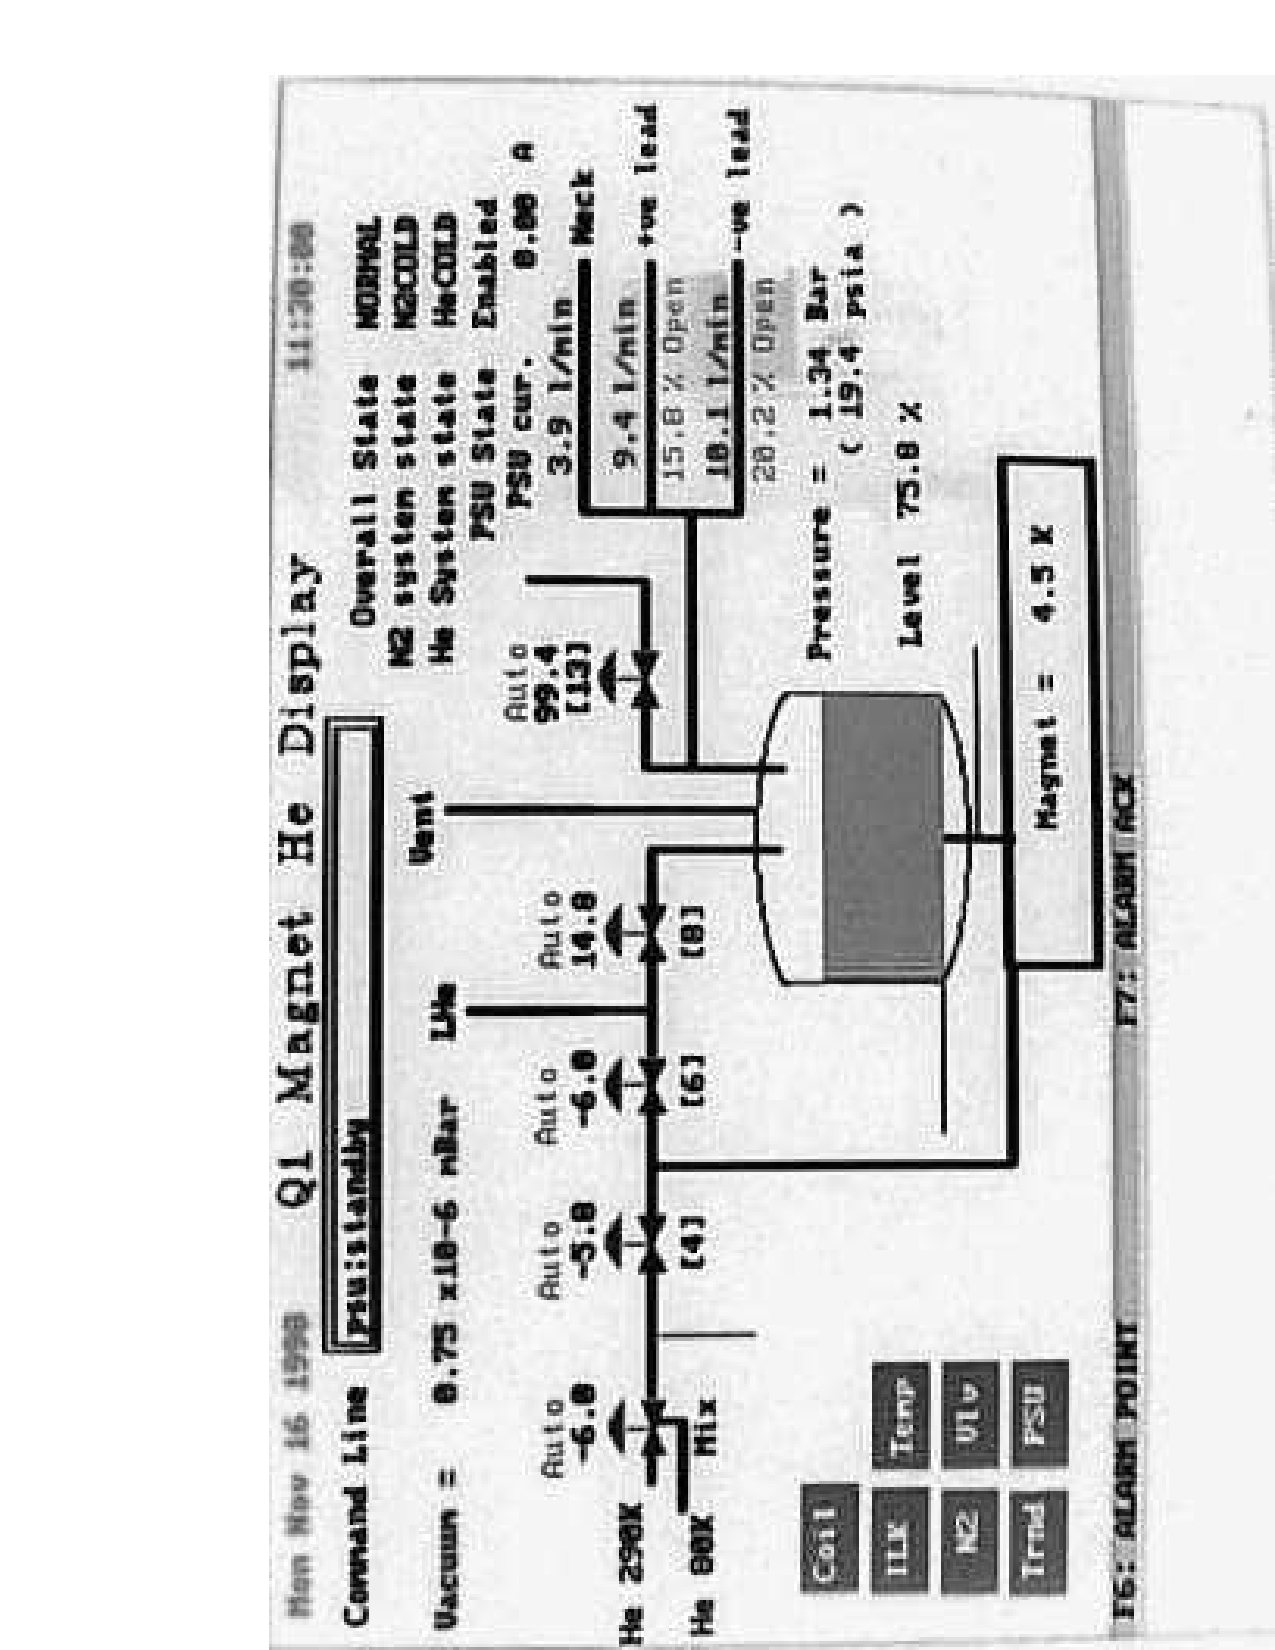
\includegraphics[angle=-90,width=4in]{Q1-helium}
\caption{Sample Helium Monitoring Page - Q1\label{fig:he_page}}
\end{figure}

\begin{figure}
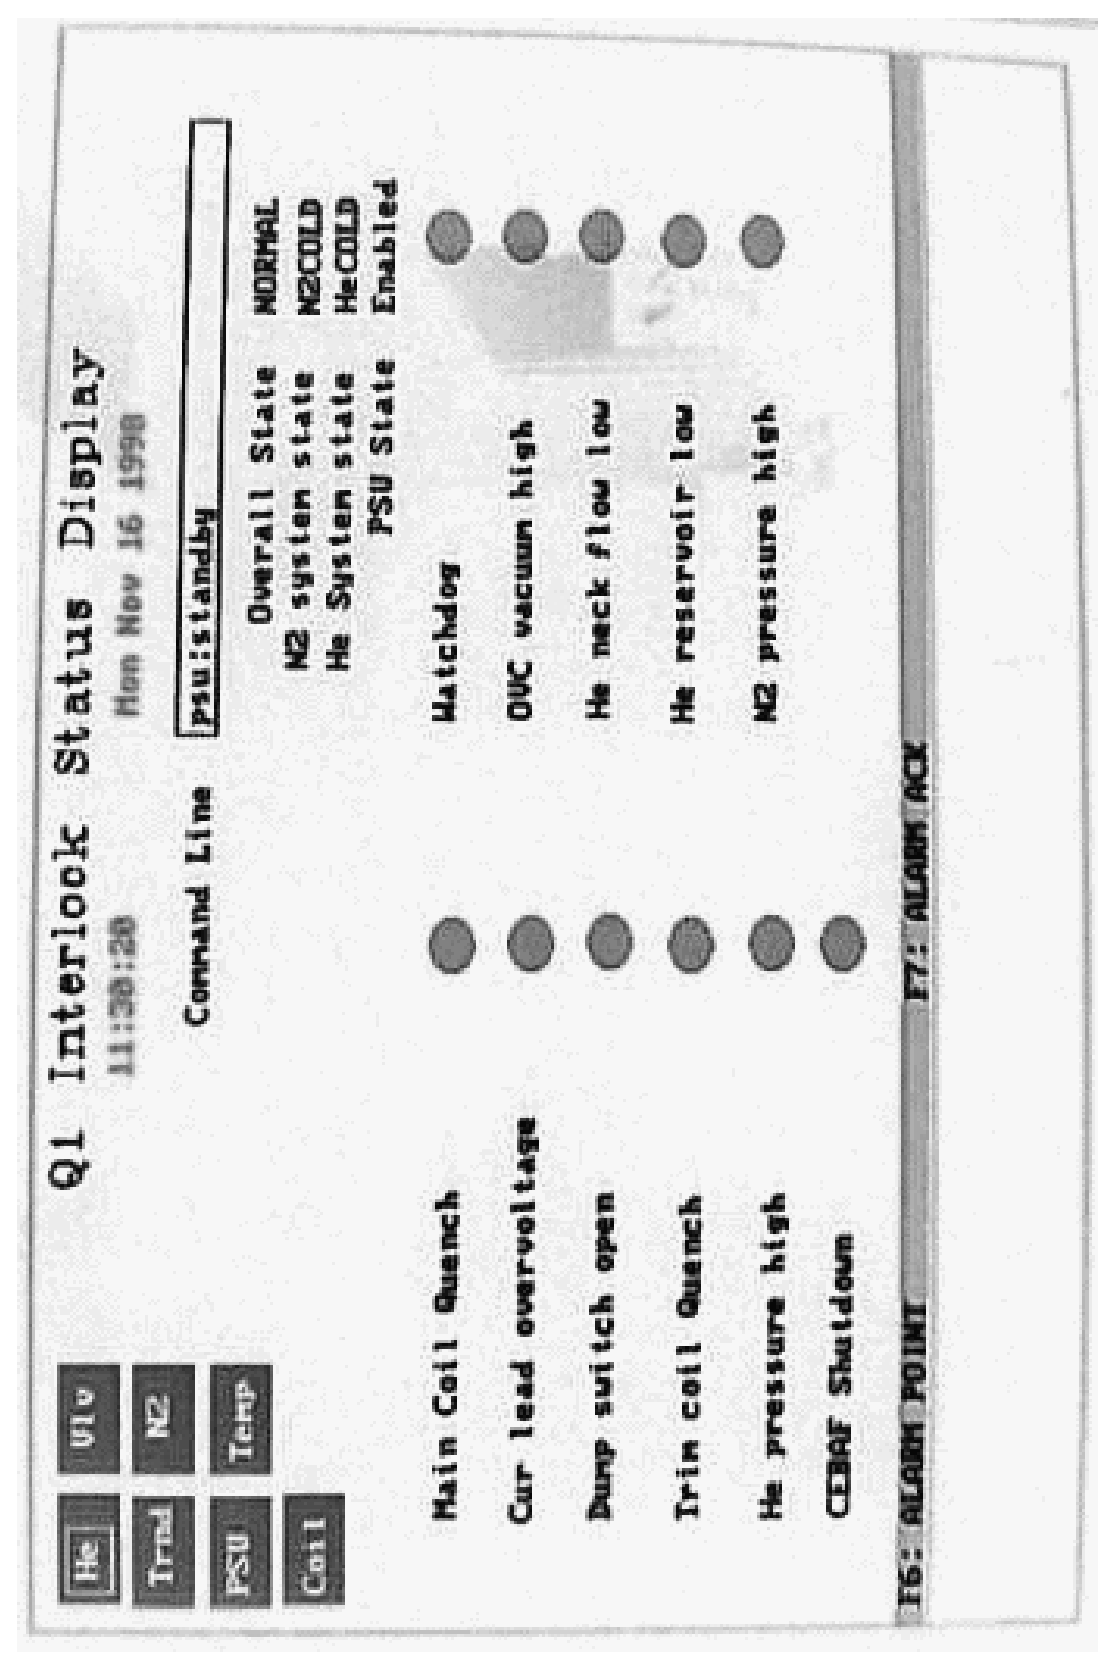
\includegraphics[angle=-90,width=4in]{Q1-interlock}
\caption{Sample Nitrogen Monitoring Page - Q1\label{fig:nit_page}}
\end{figure}

\begin{figure}
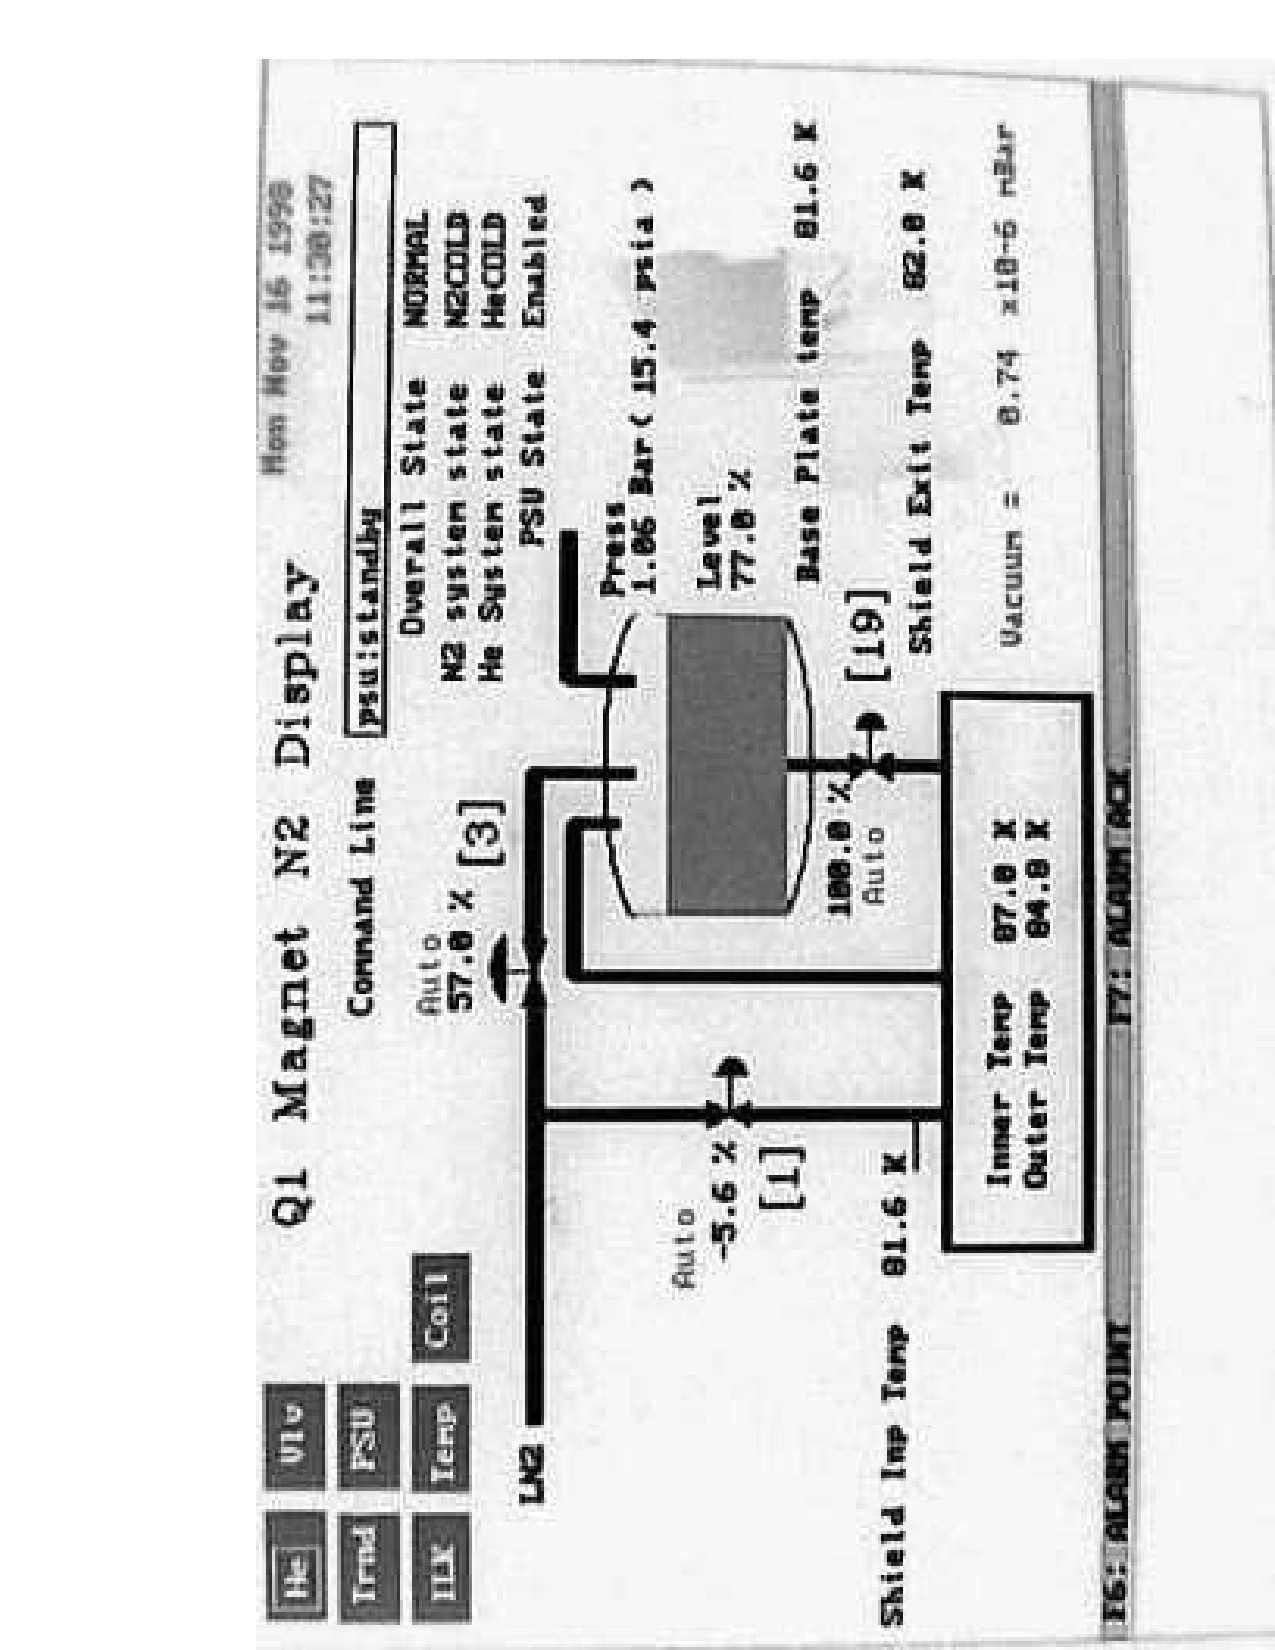
\includegraphics[angle=-90,width=4in]{Q1-n2}
\caption{Sample Power Supply Monitoring Page - Q1\label{fig:ps_page}}
\end{figure}

\begin{figure}
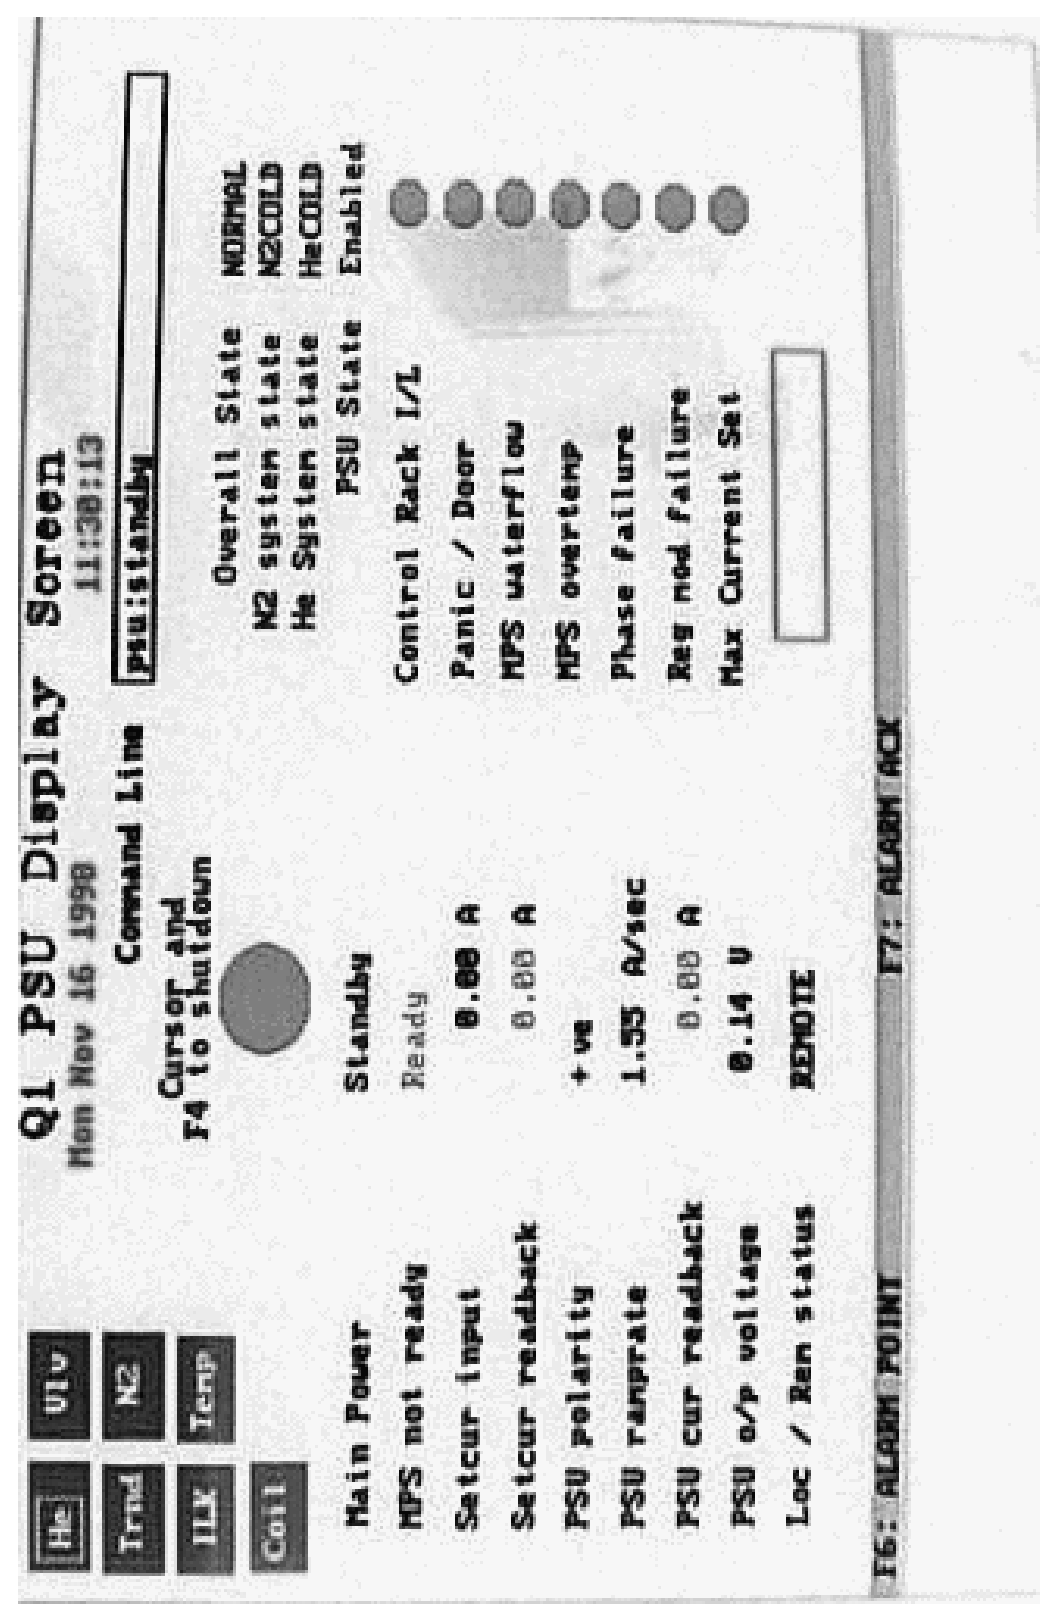
\includegraphics[angle=-90,width=4in]{Q1-psu}
\caption{Sample Interlock Monitoring Page - Q1\label{fig:is_page}}
\end{figure}

\begin{figure}
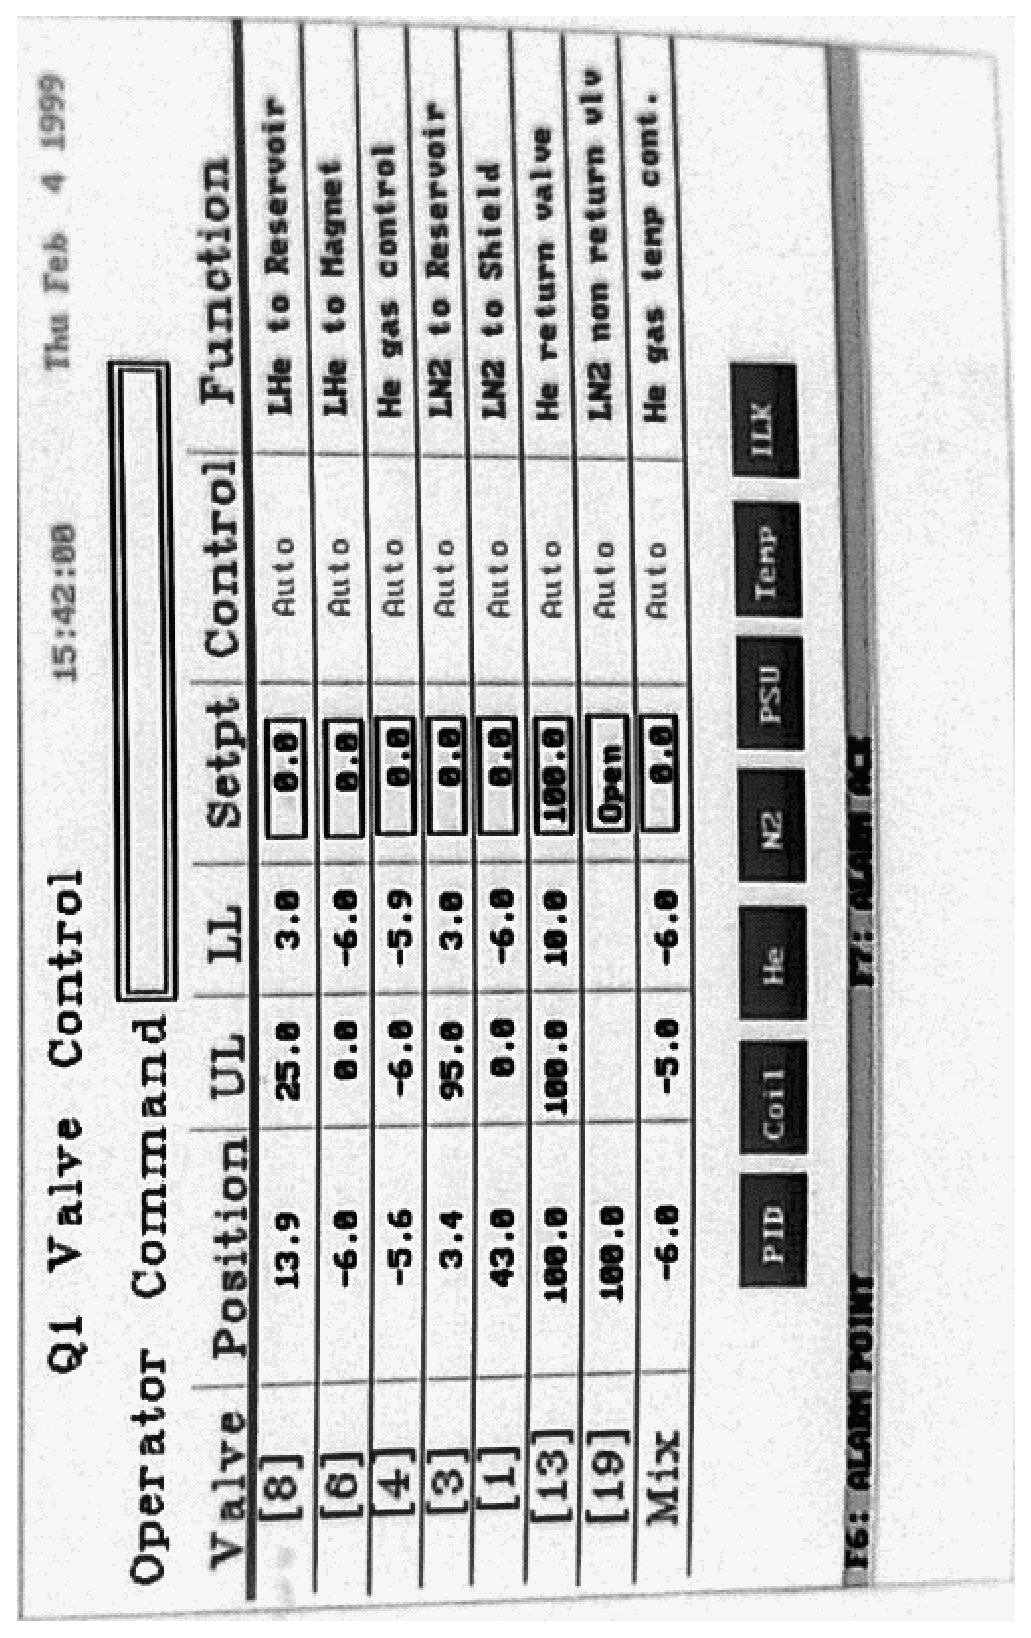
\includegraphics[angle=-90,width=4in]{Q1-valves}
\caption{Q1 Valve Control Page\label{fig:q1_valve_page}}
\end{figure}

%\begin{figure}
%\vspace{8.0in}
%\caption{Q1 Valve Control Page\label{fig:q2_valve_page}}
%\end{figure}

%\begin{figure}
%\vspace{8.0in}
%\caption{Q3 Valve Control Page\label{fig:q3_valve_page}}
%\end{figure}

\begin{figure}
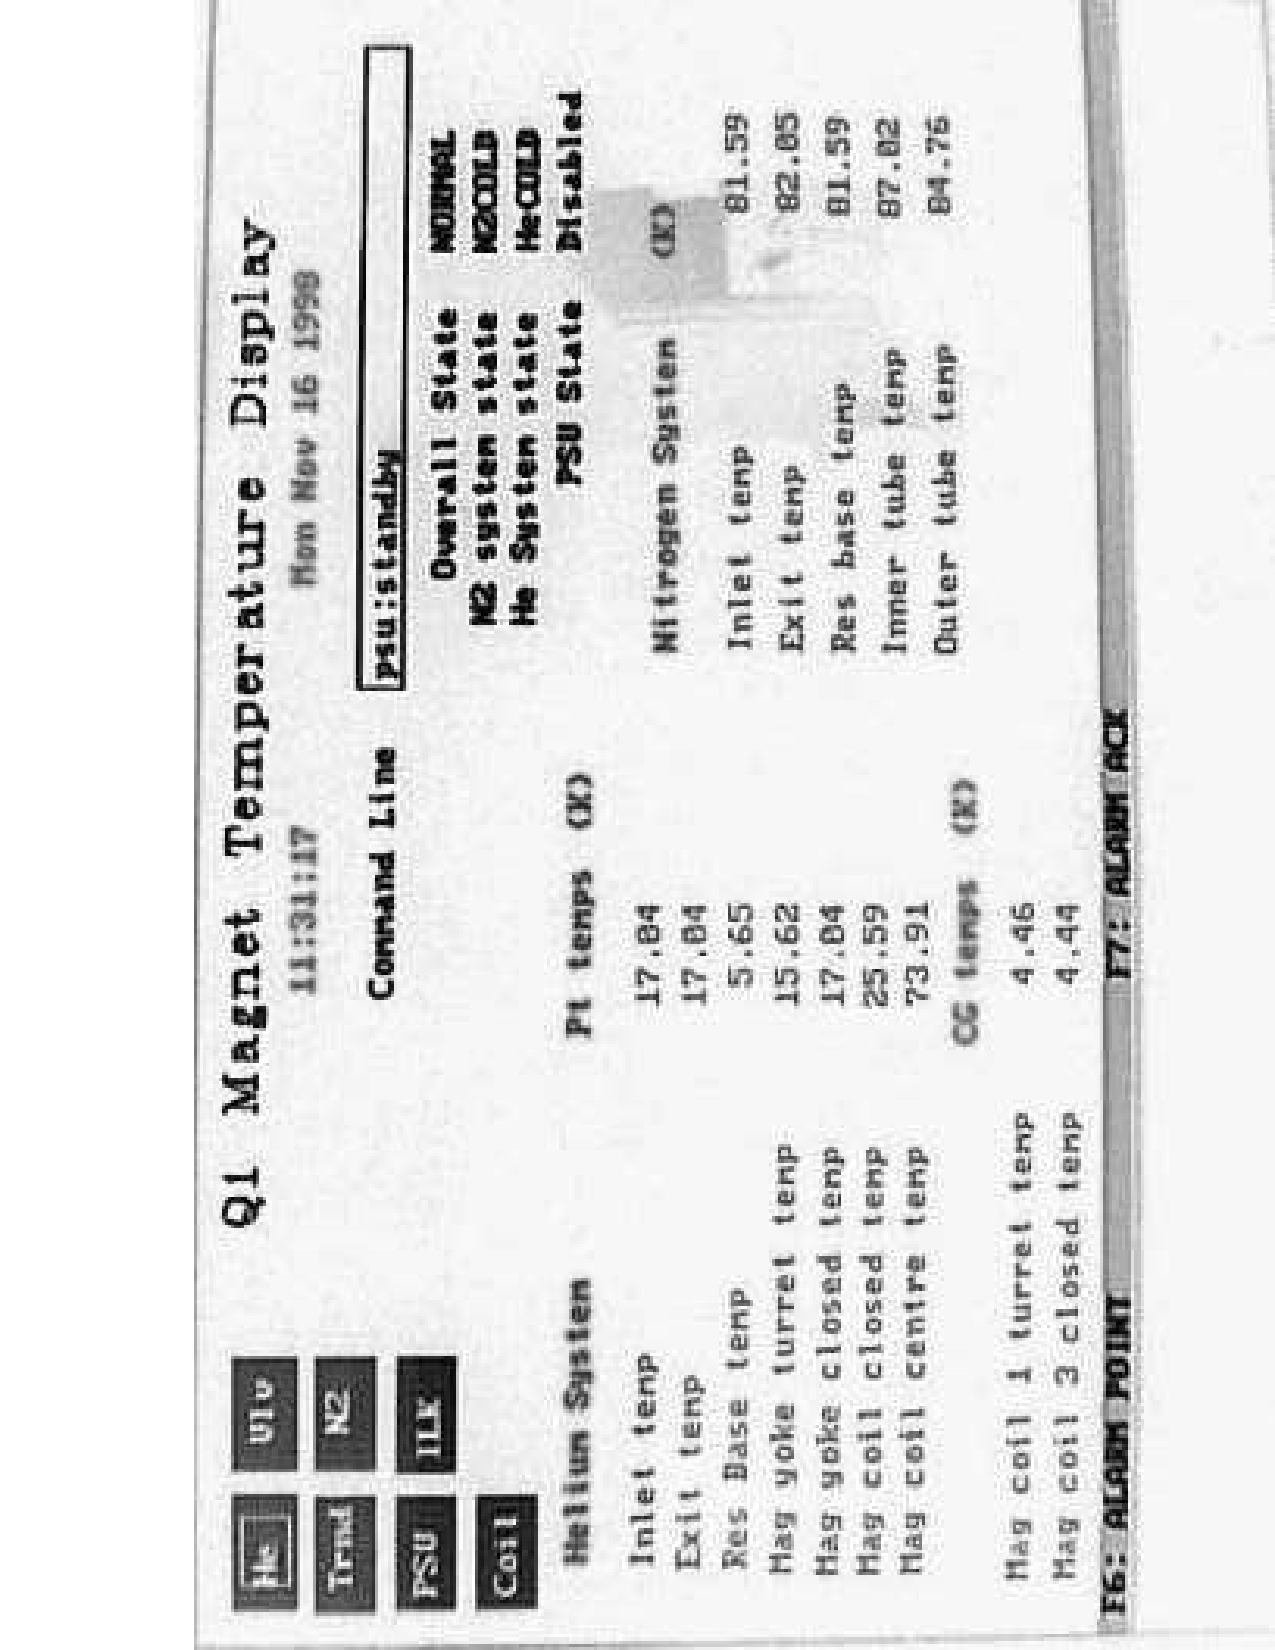
\includegraphics[angle=-90,width=4in]{Q1-temps}
\caption{Sample Magnet Temperature Display - Q1\label{fig:temp_page}}
\end{figure}

\begin{figure}
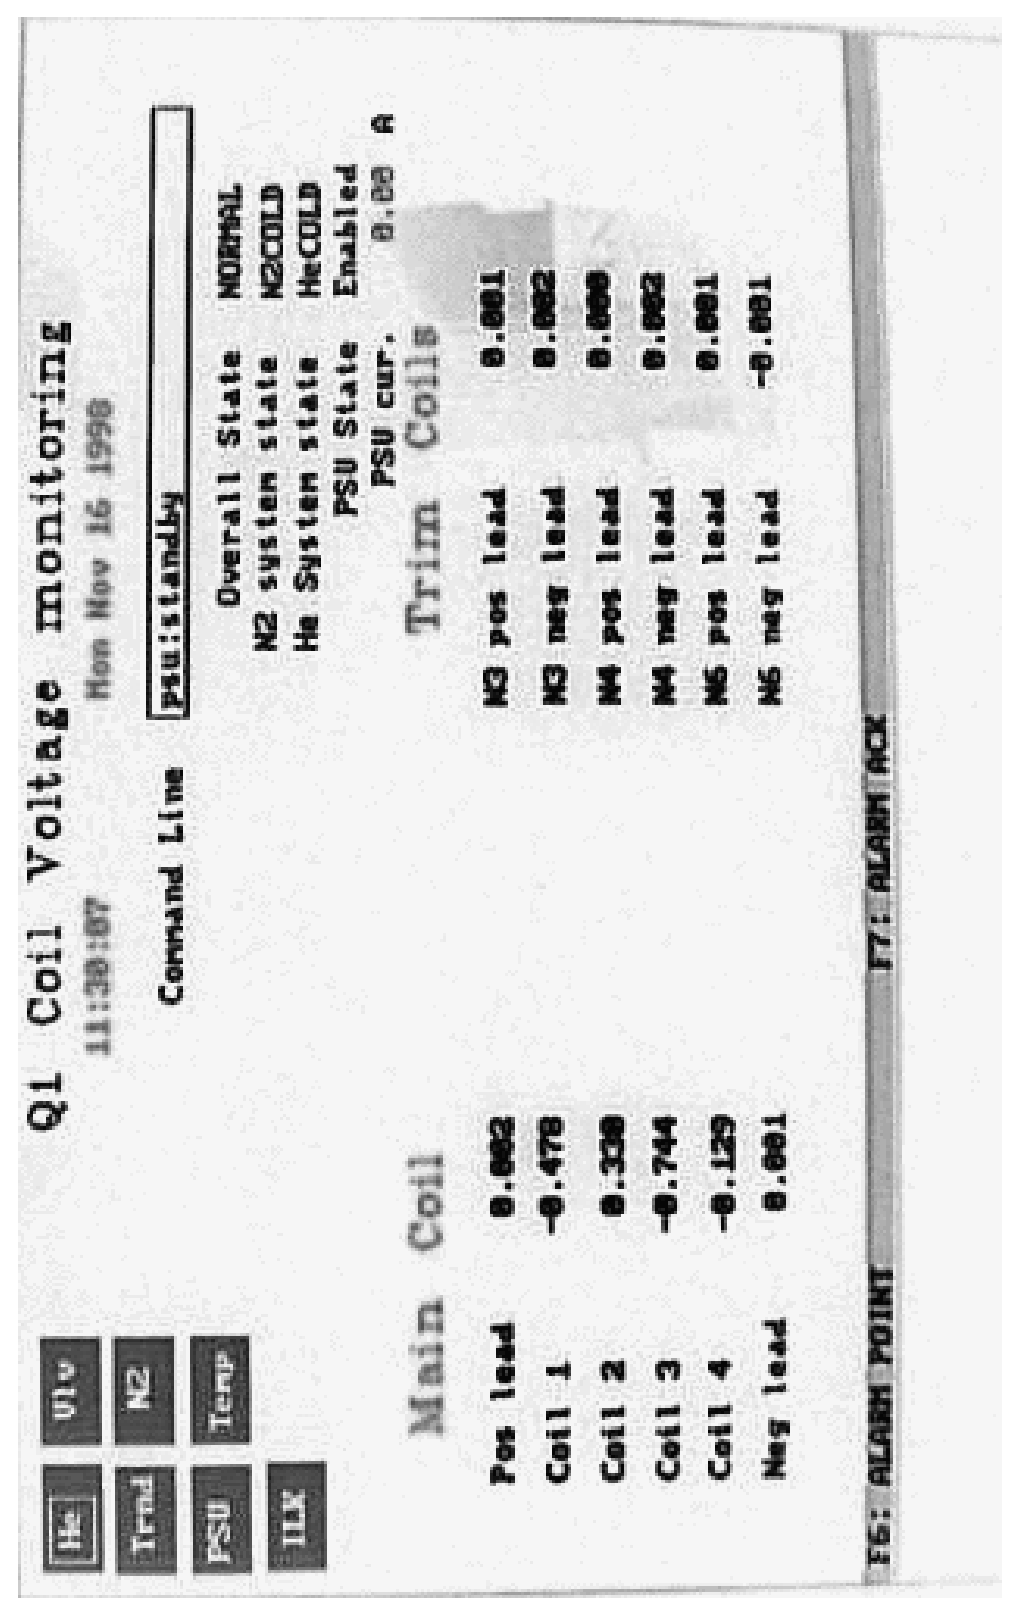
\includegraphics[angle=-90,width=4in]{Q1-voltage}
\caption{Sample Coil Voltage Monitoring Page - Q1\label{fig:coil_page}}
\end{figure}

\begin{figure}
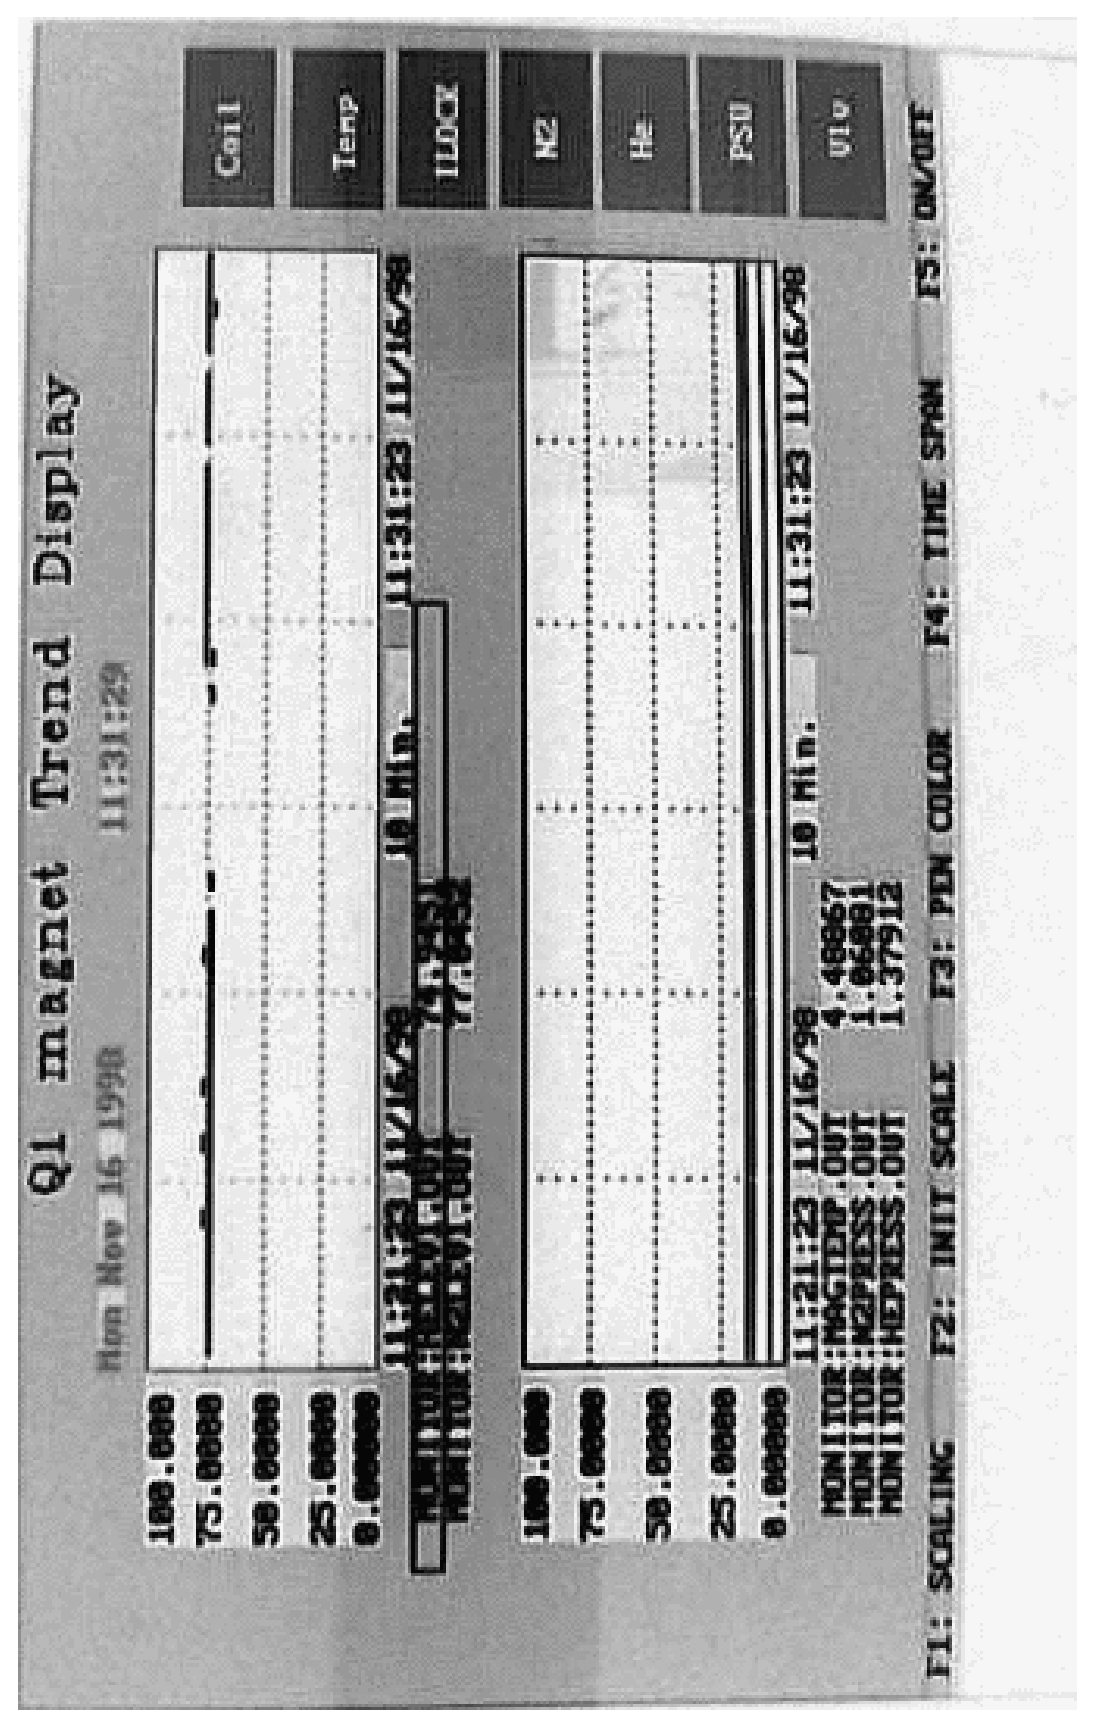
\includegraphics[angle=-90,width=4in]{Q1-trend}
\caption{Sample Trend Page\label{fig:trend_page}}
\end{figure}

\end{center}

\medskip

\begin{description}
\item[B.] {Dipole Pages}
\end{description}

\begin{description}
\item{}\hskip0.1in {[F1] Main Menu}
\item{}\hskip0.5in {Cooling (Cooldown Menu)}
\item{}\hskip0.5in {Field Regulation (NMR Controlled Programmed Ramp)}
\item{}\hskip0.5in {NMR Manual Operation (Field Control)}
\item{}\hskip0.5in {MPS Manual Operation (Current Control)}
\item{}\hskip0.1in {[F2] Coil Temperatures}
\item{}\hskip0.1in {[F3] Shield Temperatures}
\item{}\hskip0.1in {[F4] Cryogenic Page}
\item{}\hskip0.1in {[F5] Strain Gauge Page}
\item{}\hskip0.1in {[F6] Voltage Page}
\item{}\hskip0.1in {[F7] RS232 Status Page}
\end{description}


\section{HMS Vacuum System}

	The spectrometer contains five separate vacuum volumes.
These are the isolation vacuums of each of the superconducting
magnets and the main spectrometer volume through which the particles
to be detected travel.

The isolation vacuums are normally cryo pumped by the cold mass when the
magnets are cold and hence have no mechanical pumps
associated with their maintenance. They also have no thin
windows or other hazards and will not be discussed further in this document.

The main spectrometer vacuum
is currently maintained by the two mechanical pumps.
One pump is located between Q3 and the Dipole on the small angle
side of the carriage while the second pump is the backing
pump of the turbo and pumps the spectrometer volume through the turbo.
%Presently we do not use the turbo pump to pump the spectrometer volume due to
%the high leak rate through the large rear vacuum window in the shield house.
This mechanical pump is located
at the back of the carriage and the turbo is located in the shield house
underneath the end of the vacuum can that protrudes into the detector hut.

The vacuum in the spectrometer may be read out on a gauge that is sitting on the
carriage beneath Q3. There is a TV camera that views this gauge readout and
it is displayed on one of the TV monitors above the console in the hall
C counting house. The absolute value of the vacuum is not the quantity
of interest (until we improve window technology) but rather its rate of change.
Thus far we have maintained fairly stable vacuum over the course of each run
period and if things are functioning normally we should continue to do so.
If the vacuum starts to deteriorate rapidly an expert should be notified.



\section{HMS Slit System}
\label{sec:hms_slit}

The HMS slit system is installed on the gate valve housing mounted to the
front face of Q1. It consists of a vacuum box with a slit ladder
mounted into it. The slit ladder has space for three separate slits,
which will typically be one sieve slit and two solid angle defining collimators.
The slits are rectangular blocks of densimet (90\% W and 10\% Cu/Ni)
with a density of 17 g/cm$^3$. The collimators have an octagonal shaped
opening machined into them; the sieve slit has many holes drilled
into it.

The outer size of the collimators is 11.75" vertical by 8.25"
horizontal. The outer size of the sieve slit is 10.00" vertical
by 8.25" horizontal.
Its vertical size is reduced w.r.t. 11.75" due to space constraints.
The sieve slit always has to be installed at the bottom position of the ladder,
so that we can use the shielding of the collimator above it to
clearly distinguish the top row of holes. The central hole
of the sieve slit has a smaller aperture, and two blocked holes
exist to easily distinguish center and directions.
The collimator thicknesses are 2.5", while the sieve slit thickness
is 1.25". The dimensions and shape of the inner aperture of the present
HMS collimators is denoted in Table~\ref{tab:apertures}.

\begin{table}
\begin{center}
\caption{Apertures of Collimators\label{tab:apertures}}
\vspace{\baselineskip}
\begin{tabular}{|c|c|c|c|c|c|}
\hline
{} & {} & {} & {} & {} & {} \\
HMS				& d$\Omega$ 	& Horizontal 	& Vertical 		& Shape 			& Note \\
{} 				& (msr) 		& (mr) 		& (mr) 		& {} 				& {} \\
{} & {} & {} & {} & {} & {} \\ \hline
{}Need Description	& 6.74 		& $\pm$ 27.5 	& $\pm$ 70.0 	& Octagonal, Flared 	& Quads Nominal \\
{}	 			& 6.74 		& $\pm$ 27.5 	& $\pm$ 70.0 	& Octagonal, Flared 	& Quads Backward \\
{} & {} & {} & {} & {} & {} \\ \hline
%SOS & 7.55 & $\pm$ 57.5 & $\pm$ 37.5 & Octagonal, Flared & \\
%SOS & 3.98 & $\pm$ 32.5 & $\pm$ 35.0 & Octagonal, Flared & \\
SHMS			& d$\Omega$ 	& Horizontal 	& Vertical 		& Shape 			& Note \\
{} 				& (msr) 		& (mr) 		& (mr) 		& {} 				& {} \\
\hline
\end{tabular}
\end{center}
\end{table}

The total depth of the slit box is close to 3.75", which leaves
enough space to later mount scintillators behind the collimators as an active
veto counter (to prevent punch-through of hadrons) and/or to increase
the collimator thickness. Two circular quick-connect flanges are
added for feed-through of possible light guides.

A similar remotely-operated collimator box is installed on the SHMS between the
HB and Q1 magnets. The collimator ladder assembly within this box may be positioned
at three settings. The top position (accessed when the assembly is at its lowest
position) is a stretched octagon with opening height 9.843" and width 6.693" on the
upstream side. It is 2.5" thick. The lower two positions both present sieve holes in
rectangular pattern with holes separated by 0.6457" horizontally and 0.9843"
vertically. The sieve pattern at the middle ladder position has 11 columns of holes with
the sixth column centered horizontally. The holes on the bottom sieve are in ten
columns and are offset by one-half a column gap from those in the middle sieve.
The sieve collimators are 1.25" thick. The geometry is illustrated in Fig.~\ref{fig:SHMS_Collimators}.
Both sieves and octagonal collimator are
made of Mi-Tech\texttrademark{} Tungsten HD-17 (Density 17 g/cc. 90\%~W, 6\%~Ni, 4\%~Cu).

Because the SHMS has both a horizontal bend (HB magnet) and a vertical bend (main Dipole
magnet), a second sieve collimator is required for optics calibration. It is placed immediately
upstream of the HB magnet entrance. Two options are provided: a conventional passive
sieve collimator and the so-called \textit{active sieve} which is a detector based on Gas Electron 
Multipliers (GEMs).  A photo of the passive sieve options is shown in Fig.~\ref{fig:HB_Sieve_Photo}
and the dimensions and hole pattern are shown in Fig.~\ref{fig:HB_Sieve_Layout}.

\begin{figure}
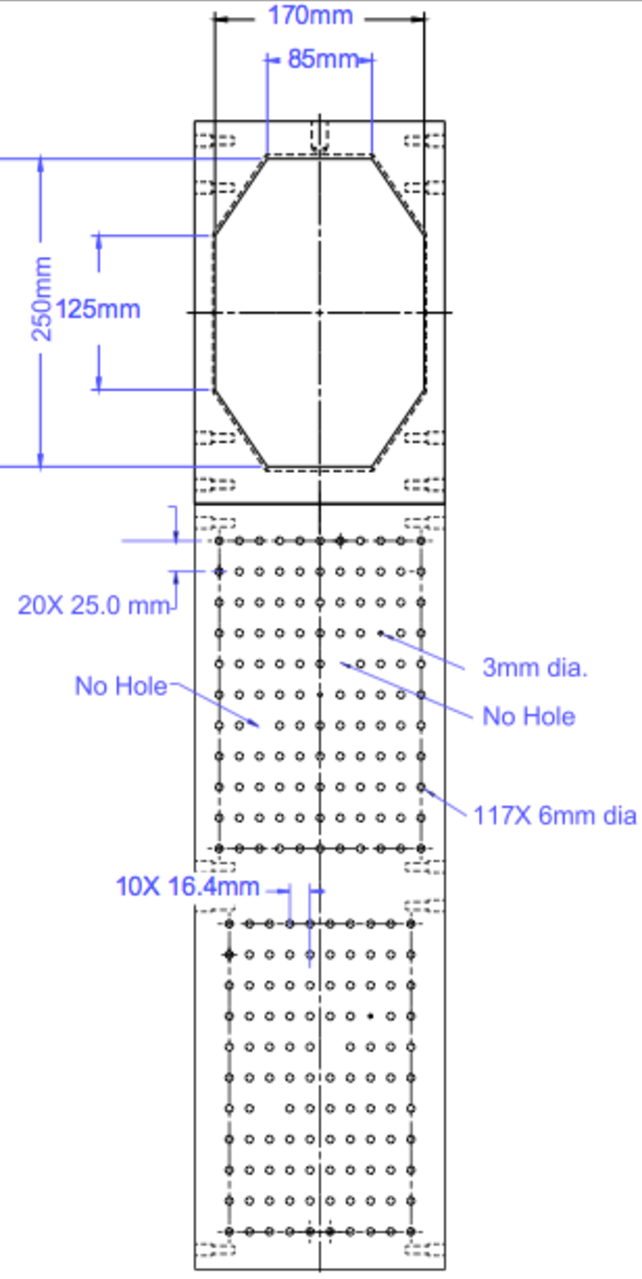
\includegraphics[width=3in]{SHMS_Collimators}
\caption{Geometry of the Main Collimator and the Sieve Slits in the SHMS \label{fig:SHMS_Collimators}}
\end{figure}

\begin{figure}
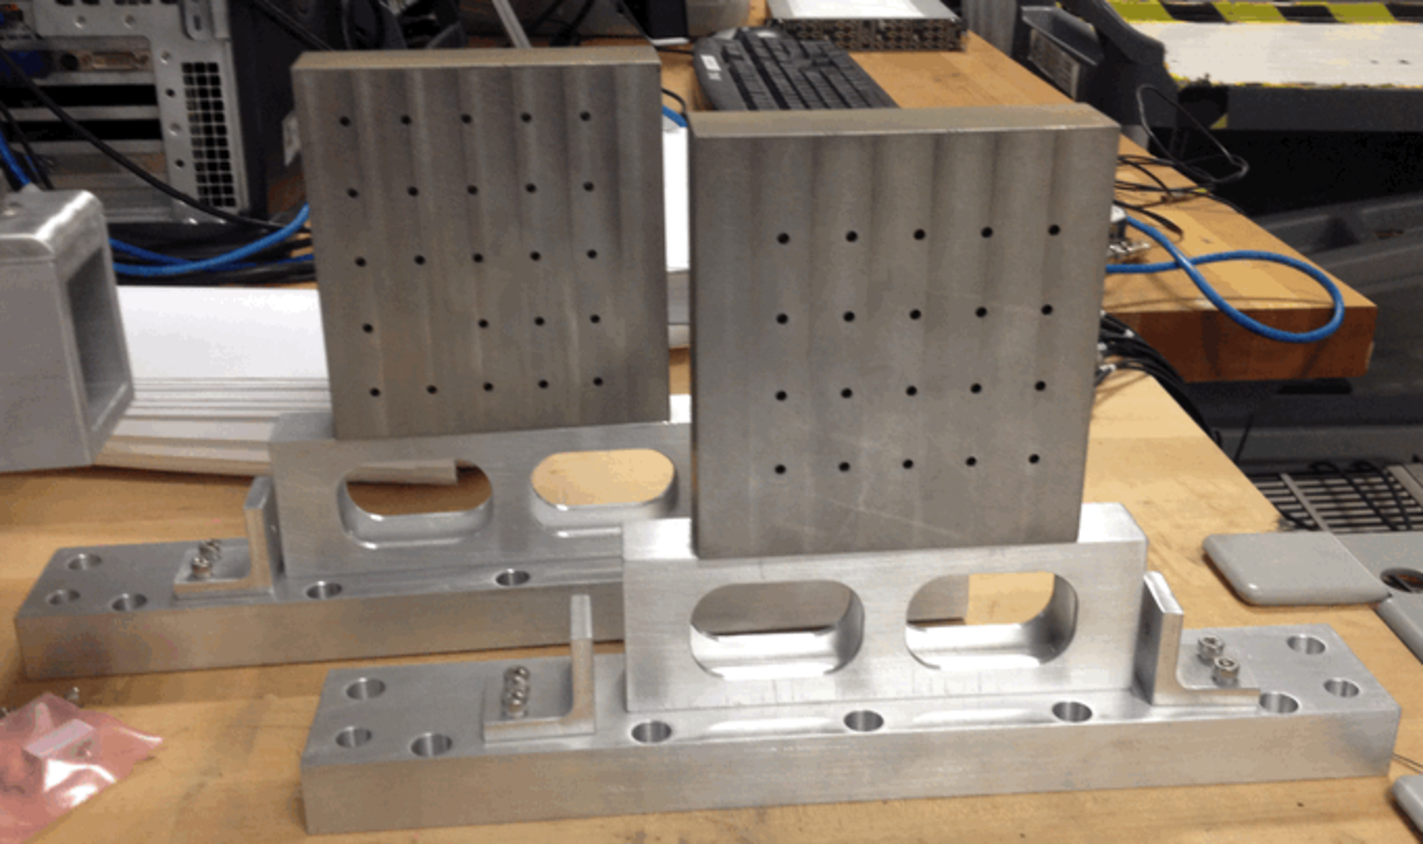
\includegraphics[width=6in]{HB_Sieve_Photo}
\caption{Upstream Sieve Slits that go on the front of the HB magnet of the SHMS \label{fig:HB_Sieve_Photo}}
\end{figure}

\begin{figure}
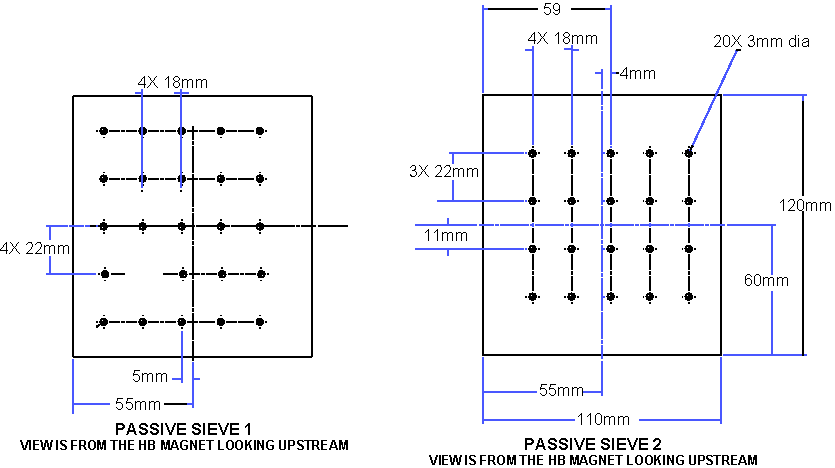
\includegraphics[width=6in]{HB_Sieve_Layout}
\caption{Upstream Sieve Slits that go on the front of the HB magnet of the SHMS \label{fig:HB_Sieve_Layout}}
\end{figure}

\subsection{Operation of the HMS Slit System}\label{sssec:slit_control}

{\bf IN 2016 EPICS DRIVERS AND SCREENS ARE BEING WRITTEN FOR 
THE COLLIMATOR MOTION CONTROLS. THE TEXT BELOW WILL NEED TO BE UPDATED.}

A remote control system consisting of motor/actuators exists to slide
the slits into place. Resolvers specify the exact position of the
slits.  The control box is located downstairs in Hall~C, behind the
blue power supply racks. On the front face there are four buttons for
each spectrometer. These indicate the three different slit positions
and the ``home" position, which denotes that no slit is used at all
(slit ladder in the up position).  Brake cables are added to prevent
the slit ladder from falling in case of a power loss. Next to this an
emergency button is included to electrically shut down the control
system.

{\bf After a power cycle the HMS slit moves itself to the {\it HOME} position,
returning a reading of 0. Thus, after a power failure or other cycle, the slit
must be commanded to a meaningful position using the commands described below.}


Normally, the system is operated remotely. Connect to the controller
using terminal server hctsv7, port 3:

\begin{minipage}{6in}
\begin{enumerate}
\item telnet hctsv7 2003
\item type \texttt{\\B} to connect to HMS, \texttt{\\A} for SOS. (Must be UPPER CASE)
\item {\tt P PFB} gives readback of the current position (see Table \ref{tab:col_pos})
\item To {\em MOVE} the collimators:
   \begin{itemize}
	\item {\tt EN} - to enable motion.
	\item {\tt RUN 10} - follow instructions (see slit numbers and postions at bottom)
	\item After you have reached the correct slit, disable the motor by typing {\tt 1}

   \end{itemize}
\item If necessary, \texttt{K} (kill) is the opposite of \texttt{EN}
\item Get rid of your session by typing \texttt{ctrl-]} (both pushed together), then
at the telnet prompt, type \texttt{quit}.
\end{enumerate}
\end{minipage}

Don't forget to get rid of your session. If you do not close your session nobody
else can communicate with the slit controllers.

%\begin{table}[!ht]\
%\caption{Slit Collimator Positions\label{tab:col_pos}}
%\begin{center}
%\begin{tabular}{rlrr}
%   &                  &     HMS   & SOS\\
%\hline
%1) & Sieve Slits      &  19804600 &  11638719\\
%2) & Large Collimator &       N/A &   3190717\\
%3) & Pion Collimator  &  -3096800 &       N/A\\
%\end{tabular}
%\end{center}
%\end{table}

\begin{table}[!ht]\
\caption{Slit Collimator Positions\label{tab:col_pos}}
\begin{center}
\begin{tabular}{rlrr}
   &                  &     HMS   & SHMS\\
\hline
1) & Sieve Slits      &  19804600 &  ????\\
2) & "Large" Collimator &       N/A &   3190717\\
3) & "Pion" Collimator  &  -3096800 &       N/A\\
\end{tabular}
\end{center}
\end{table}

   
\subsection{Hazard Identification}

The principal hazards are:
\paragraph{Magnetic:} There is a significant fringe field at
the entrance and exits of the magnets. This represents a hazard
to people working on the slit system if they are handling magnetic
objects (tools) or to people with pacemakers. In addition the field could erase magnetic
information storage media such as the strips on credit cards.
\paragraph{Mechanical:} At the front of Q1 the housing for a spring loaded gate valve is
mounted. In its normal operation mode a metal gate will be closed with
severe pressure when the electrical power drops. This can cause serious
damage to interfering body parts.  But currently the shutter and
actuator have been removed so this hazard does not exist.  
A similar mechanical problem involves the slit ladder itself. The total weight of
the three slits amounts to approximately 350 Lbs (160 Kg) and can easily
cause serious damage to body parts.

\subsection{Hazard Mitigation}

\paragraph{Magnetic}

A sign will be posted which indicates the presence of a high magnetic
field ( this is standard JLab safety signage). The exact wording is
`` High Magnetic Field - No Pacemakers or Credit Cards." There are also
flashing red lights located on the HMS carriage indicating that the
magnet power supplies are energized. Be careful with tools (are they magnetic?)
when you work on the slit boxes with the red lights in a flashing state.

\paragraph{Mechanical}

If the gate valve is ever re-installed, the following safety
procedures should be observed.  Without power, the gate valve assumes its default closed position due to
pressured air. When installing the slit boxes, or working with your hands
in the vicinity of the inside of the gate valve, disconnect first the power
plug of the gate valve, such that the gate valve closes.
In case you need the gate valve to assume a default open position without
power, first relieve the air pressure
with power on, and verify that the default position of the gate valve has
changed to ``open" by removing the power. Paul Hood (x7849) or Mike Fowler
(x7162) can be contacted for more information.

When installing the slit ladder, be careful when you work with your hands
under the slit ladder (like when you are bolting the slit box to the
gate valve). Remove the slit ladder, or {\bf install a support under the slit
ladder to prevent it from falling all the way down}.

A brake system has been included in the control to prevent the slit ladder
from sliding down in case of a power failure.  However, this must not
be relied upon for personnel safety.


\section{HMS Carriage and Rotation System }

	The Carriage is the support structure of the spectrometer.

First and foremost as it is a multi leveled structure it is important to keep in
mind that people may be working above you. 
%This means that hard hats should be worn.

There are two sets of steps on the carriage. The first set of steps
(closer to the pivot, leading to the power supplies) is very
steep (almost like a ladder) and hence extra care should be exercised
while using this set of steps. The second set of steps is at the rear
of the carriage and provides access to the main level as well as to
the catwalk and shield house. Taller individuals should be mindful
when using this flight of steps due to the limited head room at some 
points.

The first level of the carriage is almost at beam height and therefore
the usual precautions associated with working at heights should be followed (note:
safety railings have been installed everywhere possible along the carriage
perimeter, but there may still be unprotected spaces as conditions change).

The entire spectrometer can be rotated. Currently, the angle of the spectrometer
is found using a plumb bob attached to a reference mark on the
carriage frame under the ``pasta fork" at the rear of the spectrometer.
This plumb bob is aligned over survey marks which have been painted
on the floor in red and scribed at 0.5 degree intervals. Rotation of the spectrometer
is accomplished by using the two motors on the carriage itself (the motors on
the shield house bogies are not used in the present rotation system).
These AC motors are controlled by synchronous pulse width modulated
drives which are mounted near the bottom of the shield house steps.

\subsection{Remote Rotation}

Cameras are installed to enable readout of the HMS spectrometer angle
(using the plumb bob and the survey marks on the floor).

The wide-lens and zoom cameras located at the entrance and
the exit of Hall~C should be used to visually spot for obstructions
before and during remote rotation.

Limit switches are installed at forward
and backward angles which prevent HMS from rotating to angles more forward than
10.6 degrees and more backward than 85 degrees. To obtain more forward or more
backward angles an access is needed, and rotation has to occur manually
downstairs with spotters. Hard limit switches will be installed to prevent
the spectrometer from rotating out of maximum allowed range.

In case the HMS spectrometer is rotated to more forward angles, pay special
attention to possible interferences of HMS and SOS. Up to this moment
the closest  angle distance we have obtained between SOS and HMS is 28 degrees.

Remote rotation  is accomplished via the PLC located in the Hall.  It
is currently installed in the HMS shield hut for protection from
radiation.  Commands can be issued to the PLC (Texas Instruments 5000), which executes these commands
following algorithms stored in its memory. An EPICS screen is now
used to talk to the PLC.  The advantages of using the PLC are:

\begin{itemize}
\item{No direct access by users to the algorithms, preventing unsafe
rotation attempts (instead, the algorithms have to be loaded locally into
the PLC).}
\item{Rotation of both HMS and SOS by the same smart controller, enabling
security checks of both angle decoders. This renders a better handle on the
minimum allowed angle between the two spectrometers.}
\item{Automatic slower rotation speeds (if desired) if close to desired angle
when using proximity switches.}
\end{itemize}

The PLC communicates directly with the control electronics of several limit
switches, proximity switches, and decoders. Next to the limit switches
also hard limit switches will be installed on the floor to mitigate failure
of the PLC limit switches.


\subsection{Personnel Trained for Manual Spectrometer Rotation}

The spectrometer motors may only be controlled by trained personnel.
At least two people are required for spectrometer rotation, one to
run the motors and at least one spotter. Prior to rotating the spectrometer
a visual inspection of the area should be made to insure that there
is nothing in the spectrometer's path or on the rails. During rotation
the spotter should pay special attention to
the cables which run from the
spectrometer to the target motor controller to make sure that
nothing is hung up or stretching.

In case you need to rotate the spectrometer manually, contact one of the trained
personnel listed in Responsible Personnel (chapter 4) in
the \htmladdnormallinkfoot{ESAD}{http://www.jlab.org/Hall-C/document}.
}

\infoleveqnull{\section{Spectrometer Rotation}

\sawnote{This section is just for the ESAD.  Currently just based on the
Hall A ESAD.  The HMS rotation discussion above needs to be updated
and broadened to also include the SHMS and this ESAD text merged in.
Include statement that angle limits are set by experiment and that
movements to small angles may need to be done by experts.
}


%
%
Since the Hall C spectrometers each weigh in excess of \sawnote{XXX}
tons it is very important that all safety precautions are carefully
adhered to.   During operations, the spectrometers are certified
to allow remote rotation by shift crews within prescribed limits.  In
the absence of this certification, the spectrometers may only be
rotated by trained technical staff.

\begin{safetyen}{0}{0}
\subsection{Hazards}

Hazards include:
\begin{itemize}
\item{Knocking items over.}
\item{The wheels crushing things (including fingers and toes) on the floor in the path of the 
spectrometer}
\item{Damaging the beamline or other equipment on the floor if one goes to too small 
or too large an angle, or if it just gets pushed around inadvertently.}
\item{Tearing out of cables etc. physically attached to the superstructure}
\end{itemize}

\subsection{Mitigations}

Hazard mitigations:
\begin{itemize}
\item{Stop-blocks attached to the rails to prevent spectrometer rotation beyond the needed angular range.}
\item{Audible alarm on the spectrometers indicating they are in motion or that motion
is possible (controls engaged etc.)}
\item{During a running experiment the run coordinator and work coordinator should know in advance 
of any moves.  Moves at any other time must be cleared with the Hall work coordinator 
before implementation.}
\item{Careful inspection of the intended path to make sure it is clear. This is part of
the pre-run checklist performed by the technical staff prior to closing the Hall and
a remote camera allows shift worker to inspect the area.}
\item{Any motion that takes a spectrometer inside 14 degrees or outside \emph{X} degrees
(\emph{X} being specified in the pre-run checklist and noted on the whiteboard during a run) 
must be supervised by a trained Hall C technician.}
\end{itemize}
\end{safetyen}

\subsection{Responsible Personnel}

Following the experimental run plan, as posted in the counting house
by the run coordinator, shift workers are allowed to rotate the HRS
following guidelines of the standard equipment manual.  In the event
of a problem getting the spectrometers to rotate the run coordinator
should notified.  If the run coordinator is unable to solve the
problem, and with the run coordinators concurrence, qualified
personnel should be notified to repair the problem (see
Table~\ref{tab:spectrometers:personnel_rotate}).  On weekends and after hours
please only use the tech-on-call number.  It should be noted that for
experiments that are using thick targets at high current, it is not
uncommon that the produced radiation will cause the motion system to
require a hard reset.

\begin{namestab}{tab:spectrometers:personnel_rotate}{Spectrometer Rotation: authorized personnel}{%
      List of HRS responsible personnel where ``W.B.'' stands for the white board 
      in the counting house.}
   \TechonCall{\em Contact}
   \MikeFowler{}
   \WalterKellner{}
   \AndyKenyon{}
   \JoeBeaufait{}
\end{namestab}

}
